\documentclass[]{tukediphc}
%% -----------------------------------------------------------------
%% tento subor ma kodovanie utf-8
%%
%% na kompilaciu pouzivajte format pdfcslatex 
%%
%% vytvorene distribuciou texlive 2009-7, OS GNU/Linux
%% vytvorene distribuciou TeXLive 2010, OS Win XP
%% februar 2013
%% -----------------------------------------------------------------
\usepackage[utf8]{inputenc}
%\usepackage[T1]{fontenc}
\usepackage{lmodern,textcase}
\usepackage{slovak}\renewcommand{\figurename}{Obr\'azok}
\def\refname{Zoznam pou\v{z}itej literat\'ury}
\usepackage{latexsym}
\usepackage{dcolumn} % zarovnanie cisiel v tabulke podla des. ciarky
\usepackage{hhline}
\usepackage{amsmath}
\usepackage{nicefrac} % pekne zlomky
\usepackage{upgreek} % napr. $\upmu\mathrm{m}$ pre mikrometer ...
\usepackage[final]{showkeys}%color%notref%notcite%final
\usepackage[slovak,noprefix]{nomencl}
\makeglossary % prikaz na vytvorenie suboru .glo
\usepackage{parskip}% 'zhusti' polozky obsahu
%%
%\usepackage[dvips]{graphicx}
%\DeclareGraphicsExtensions{.eps}
\usepackage[pdftex]{graphicx}
\DeclareGraphicsExtensions{.pdf,.png,.jpg,.mps}
\graphicspath{{figures/}} % priecinok na obrazky
%%
%% Cislovane citovanie
%\usepackage[numbers]{natbib}
%\usepackage{pdfpages}%spoji vystupne pdfko s dalsim pdfkom <-pre zadavaci list
%%
%% Citovanie podľa mena autora a roku
\usepackage{natbib} \citestyle{chicago}
% -----------------------------------------------------------------
%% tlač !!!
\usepackage[pdftex,unicode=true,bookmarksnumbered=true,
bookmarksopen=true,pdfmenubar=true,pdfview=Fit,linktocpage=true,
pageanchor=true,bookmarkstype=toc,pdfpagemode=UseOutlines,
pdfstartpage=1]{hyperref}
\hypersetup{%
baseurl={http://www.tuke.sk/sevcovic},
pdfcreator={pdfcsLaTeX},
pdfkeywords={Sprostredkovanie, Medi\'ator, IPFIX, SLAMeter, BasicMeter},
pdftitle={Aplikačný rámec pre sprostredkovanie IPFIX správ v nástroji SLAmeter},
pdfauthor={Bc. Rastislav Kudla},
pdfsubject={Diplomová práca}
} 
%% nehodiace zakomentujte !
\dippraca{Diplomová práca}
%\bakpraca{Bakalárska práca}
%%
\nazov{Aplikačný rámec pre sprostredkovanie IPFIX správ v nástroji SLAmeter}
%% ked praca nema 'podnazov' zakomentujte nasledujuci riadok
%% alebo polozku nechajte prazdnu
\podnazov{}
\autor{Bc. Rastislav Kudla}
\veduciprace{Ing.~Peter~Feciľak, PhD.}
\konzultanta{Ing.~Adrián~Pekár}
%\konzultantb{RNDr.~Marián~Čierny, DrSc.}
\univerzita{Technická univerzita v~Košiciach}
\fakulta{Fakulta elektrotechniky a informatiky}
\skratkafakulty{FEI}
\katedra{Katedra počítačov a informatiky}
\skratkakatedry{KPI}
\odbor{Informatika}
\specializacia{Informatika}

\abstrakt{Abstrakt je povinnou súčasťou každej práce. Je výstižnou
charakteristikou obsahu dokumentu. Nevyjadruje hodnotiace stanovisko
autora. Má byť\/ taký informatívny, ako to povoľuje podstata práce.
Text abstraktu sa píše ako jeden odstavec. Abstrakt neobsahuje odkazy
na samotný text práce. Mal by mať\/ rozsah 250 až 500 slov. Pri
štylizácii sa používajú celé vety, slovesá v činnom rode a tretej
osobe. Používa sa odborná terminológia, menej zvyčajné termíny,
skratky a~symboly sa pri prvom výskyte v texte definujú.}

\klucoveslova{Sprostredkovanie, Mediátor, Kolektor, Exportér, IPFIX, SLAMeter, BasicMeter}

\abstrakte{Text abstraktu v~svetovom jazyku je potrebný pre integráciu
do medzinárodných informačných systémov. Ak nie je možné cudzojazyčnú
verziu abstraktu umiestniť na jednej strane so slovenským abstraktom,
je potrebné umiestniť ju na samostatnú stranu (cudzojazyčný abstrakt
nemožno deliť a~uvádzať na dvoch strabách).}

\keywords{Mediation, Mediator, Collector, Exporter, IPFIX, SLAMeter, BasicMeter}

\datumodovzdania{26. 4. 2013}
\mesto{Košice}


%----------ZOZNAM SKRATIEK-------------------
\nomenclature{IETF}{Internet Engineering Task Force}
\nomenclature{IP}{Internet Protocol}
\nomenclature{IPv4}{Internet Protocol verzie 4}
\nomenclature{IPv6}{Internet Protocol verzie 6}
\nomenclature{ISP}{Internet Service Provider}
\nomenclature{IANA}{Internet Assigned Numbers Authority}
\nomenclature{PEN}{Private Enterprise Number}
\nomenclature{LAN}{Local Area Network}
\nomenclature{UTC}{Coordinated Universal Time}
\nomenclature{IPFIX}{IP Flow Information eXport}
\nomenclature{MONICA}{Monitoring and Optimization of Network Infrastructures Communications and Applications}
\nomenclature{napr.}{napríklad}
\nomenclature{a pod.}{a podobne}
\nomenclature{atd.}{a tak dalej}
\nomenclature{resp.}{respektívne}
\nomenclature{Gb/s}{Gigabit za sekundu}
\nomenclature{BGP}{Border Gateway Protocol}
\nomenclature{ID}{Identification (number)}
\nomenclature{CNL}{Computer Networks Laboratory}
\nomenclature{BEEM}{BasicMeter Exporting and Measuring process}
\nomenclature{JXColl}{Java XML Collector}
\nomenclature{ACP}{Analyzer-Colector Protocol}
\nomenclature{SQL}{Structured Query Language}
\nomenclature{ECAM}{Exporter-Collector-Analyzer Manager}
\nomenclature{BMAnalyzer}{BasicMeter Analyzer}
\nomenclature{XML}{eXtensible Markup Language}
\nomenclature{UDP}{User Datagram Protocol}
\nomenclature{TCP}{Transmission Control Protocol}
\nomenclature{SCTP}{Stream Control Transmission Protocol}
\nomenclature{SLAmeter}{Service-level agreement metering}
\nomenclature{bmIDS}{BasicMeter Intrusion Detection System}
\nomenclature{FIFO}{First-In-First-Out}
\nomenclature{JVM}{Java Virtual Machine}
\nomenclature{JRE}{Java Runtime Environment}
\nomenclature{JDK}{Java Development Kit}
\nomenclature{MAC}{Media Access Control}
%----------------DELENIE SLOV-------------
%\hyphenation{IPFIXFlowRecord FlowRecordDispatcher}

%-----------------------------------------

\begin{document}
\renewcommand\theHfigure{\theHsection.\arabic{figure}}
\renewcommand\theHtable{\theHsection.\arabic{table}}
\bibliographystyle{dcu}

\prvastrana

\titulnastrana

\abstraktsk % abstrakt v SK 

\abstrakteng % abstrakt v ENG

\kabstrakt % koniec abstraktov, nova strana

% Na tomto mieste bude vložené zadanie diplomovej práce
%\includepdf[pages=-]{zadavaci_list_gray.pdf} 
\zadanieprace

\cestnevyhlasenie
% Niektorí autori metodických príručiek o~záverečných prácach sa
% nazdávajú, že takéto vyhlásenie je zbytočné, nakoľko povinnosť
% vypracovať záverečnú prácu samostatne, vyplýva študentovi zo zákona a
% na autora práce sa vzťahuje autorský zákon.

\podakovanie
Na tomto mieste sa chcem poďakovať vedúcemu diplomovej práce Ing. Petrovi 
Feciľakovi, PhD., konzultantovi Ing. Adriánovi Pekárovi ako aj členom 
výskumnej skupiny MONICA za ich ochotu, cenné
rady, pripomienky a odbornú pomoc pri riešení diplomovej práce.

Obzvlášť veľká vďaka patrí mojej rodine a najbližším za podporu a pomoc 
počas celého štúdia na vysokej škole.
\kpodakovania

\predhovor
Predhovor je povinnou náležitosťou záverečnej práce, pozri
\citep{gonda}. V~predhovore autor uvedie základné charakteristiky
svojej záverečnej práce a~okolnosti jej vzniku. Vysvetlí dôvody, ktoré
ho viedli k~voľbe témy, cieľ a~účel práce a~stručne informuje
o~hlavných metódach, ktoré pri spracovaní záverečnej práce použil.
\kpredhovoru

\thispagestyle{empty}
\tableofcontents
\newpage

\thispagestyle{empty}
%\addcontentsline{toc}{section}{\numberline{}Zoznam obrázkov}
\listoffigures
\newpage

\thispagestyle{empty}
%\addcontentsline{toc}{section}{\numberline{}Zoznam tabuliek}
\listoftables
\newpage

\thispagestyle{empty}
%\addcontentsline{toc}{section}{\numberline{}Zoznam symbolov a
%skratiek}
\printglossary % vlozenie zoznamu skratiek a symbolov
\newpage

%\addcontentsline{toc}{section}{\numberline{}Slovník termínov}
\slovnikterminov

\begin{description}
	
	\item[Unix Timestamp] nazývaný tiež Unix time, alebo POSIX time je systém na vyjadrovanie 
	hodnoty času. Je definovaný ako počet uplynutých sekúnd od polnoci 1. januára 1970 UTC.
	
	\item[Singleton] je návrhový vzor, ktorý povoľuje vytvorenie iba jednej inštancie triedy. 
	
	\item[Parser] je program, ktorý analyzuje vstupne dáta tak, že ich rozdelí na jednotlivé 
	významové časti, ktoré môžu byť následne spracované. \citep{veri}
	
	\item[Paket] je forma, resp. blok binárnych dat prenášaných v počítačových sieťach.
	
	\item[Hash mapa] alebo hash tabuľka je dátová štruktúra používaná na implementáciu asociatívnych 
	poli. K hashovacim kľúčom priraďuje zodpovedajúce hodnoty. V jazyku Java môže byť hodnotou 
	akýkoľvek objekt a kľúčom každý objekt, ktorý správne implementuje funkcie \emph{equals()} a 
	\emph{hashCode()}.
	
	\item[IPv4 adresa] je 32 bitové označenie zariadenia v počítačovej sieti, ktoré na komunikáciu 
	používa Internet Protocol verzie 4 \citep{rfc791}.
	
	\item[IPv6 adresa] je 128 bitové označenie zariadenia v počítačovej sieti, ktoré na komunikáciu 
	používa Internet Protocol verzie 6 \citep{rfc2460}.
	
	\item[MAC adresa] je 48 bitový, unikátny identifikátor sieťového adaptéra komunikujúceho na 
	fyzickej vrstve. 
	
	\item[Big-Endian] je spôsob usporiadania bytov dátových typov v pamäti počítača. Najvýznamnejší 
	byte je uložený na najnižšej (prvej) pozícii. Používa sa pri komunikácii v počítačových sieťach,
	preto sa tiež nazýva \uv{sieťové poradie bytov}. Jeho presným opakom je Little-Endian.
	
	\item[Buffer] je oblasť pamäte používaná na dočasné uchovanie dát pred ich presunom na iné 
	miesto - vyrovnávacia pamäť.
	
	\item[paket]
	\item[soket]
	
\end{description}

\kslovnikterminov
%
\setcounter{page}{1}
\setcounter{equation}{0}
\setcounter{figure}{0}
\setcounter{table}{0}

\section*{\'Uvod}
\addcontentsline{toc}{section}{\numberline{}\'Uvod}

Rozmach počítačových sietí prináša ľudstvu nové možnosti a služby, o~akých sme kedysi ani nesnívali.
Internet sa stal súčasťou nášho každodenného života, mnohí sú pripojení aj 24 hodín denne, nielen 
prostredníctvom počítačov, ale aj mobilných zariadení. Práve vďaka rozmachu mobilného Internetu si už
ani nevieme predstaviť situáciu, že by sme neboli v~dosahu Internetového obsahu. Týmto sú kladené 
obzvlášť vysoké nároky na kvalitu sietí a poskytovaných služieb. Aby poskytovatelia Internetu mohli 
zabezpečovať a zlepšovať kvalitu služieb (QoS), musia ju vedieť merať.

V~Laboratóriu počítačových sietí \emph{(CNL)} na Technickej univerzite v~Košiciach vyvíja výskumná 
skupina MONICA pasívny merač parametrov sieťovej prevádzky na~báze tokov, ktorý vyhodnocuje 
dodržiavanie zmluvy o~úrovni poskytovanej služby \emph{(SLA)}. Jeho cieľom je spracovať určité parametre 
sieťovej prevádzky a na ich základe vypočítať triedu kvality. Táto aplikácia má slúžiť nielen poskytovateľom 
pripojenia k~Internetu ako monitorovací nástroj. Triedy umožňujú aj ich klientom jednoducho 
porovnávať kvalitu poskytovaných služieb. Jadro nástroja SLAmeter sa skladá z~komponentov, ktoré sú 
navrhnuté v~súlade s~protokolom IPFIX. \citep{slameter}

Komponentmi architektúry IPFIX \emph{(IP Flow Information Export)} podľa RFC 5470 \citep{rfc5470}
sú exportéry a kolektory komunikujúce protokolom IPFIX. Vzhľadom k~trvalému rastu IP prevádzky
v~heterogénnych sieťových prostrediach, tieto exportér-kolektor systémy môžu viesť k~problémom 
škálovateľnosti. Ba čo viac, neposkytujú flexibilitu potrebnú pre široký rad meracích aplikácií.

Pre naplnenie požiadaviek aplikácií s~obmedzenými systémovými zdrojmi, IPFIX architektúra zavádza 
sprostredkovateľskú entitu medzi exportéry a kolektory. Z~pohľadu manipulácie s~dátami môžu sprostredkovateľské
moduly tejto entity poskytovať agregáciu, koreláciu, filtrovanie, selekciu, anonymizáciu a iné úpravy záznamov o~
tokoch za účelom 
šetrenia výpočtových zdrojov meracieho systému a vykonávania predspracovania úloh pre kolektor. Z~hľadiska
interoperability nástrojov rôznych vývojárov, môžu poskytovať konverziu z~iných protokolov na IPFIX, 
respektíve zvyšovať spoľahlivosť exportov napríklad prevodom z~nespoľahlivého, bezspojovo orientovaného 
protokolu UDP na spoľahlivý SCTP. \citep{rfc6183}

Táto práca analyzuje nastolený problém sprostredkovania správ a sprostredkovateľských entít nazývaný 
\emph{IP Flow Information Export (IPFIX) Mediation Problem}. Jej hlavným cieľom je navrhnúť a implementovať
aplikačný rámec pre sprostredkovateľskú entitu zvanú IPFIX Mediátor pre účely nástroja SLAmeter. 
Rámec musí klásť veľký dôraz na jeho modularitu, aby bolo jednoduché a pohodlné implementovať nové 
sprostredkovateľské moduly a tým zvyšovať možnosti monitorovania aplikáciou SLAmeter.

Štruktúra práce je nasledovná. V~úvodnej kapitole je formulovaná definícia úlohy. Druhá kapitola sa 
v~krátkosti venuje protokolu IPFIX. Popisuje len formát IPFIX správy, jej hlavičku, typy
sád a ich komponenty. Ostatné rysy protokolu si môže čitateľ vyhľadať v~príslušných dokumentoch RFC.
Nasledujúca podrobne analyzuje problém sprostredkovania správ v~IPFIX. Úvodom definuje použitú 
terminológiu. Analyzuje nevýhody exportér-kolektor architektúr bez Mediátora, príklady použitia 
sprostredkovania, ale aj jeho implementačno-špecifické problémy. Ďalšia sekcia sa zaoberá analýzou 
aplikačného rámca pre IPFIX Mediátor. Tretia kapitola stručne priblíži projekty výskumnej skupiny MONICA.
Nasledujúca kapitola s~poradovým číslom štyri, tvorí jadro práce. V~nej sa čitateľ dočíta o~návrhu a 
implementácii aplikačného rámca pre sprostredkovateľskú entitu. Jednotlivým triedam a metódam vyššieho 
významu je venované podrobné vysvetlenie. Predposledná kapitola niekoľkými testami experimentálne 
overuje implementované riešenie. Záver už len zhodnotí diplomovú prácu a jej dosiahnuté výsledky. 


%V~úvode autor podrobnejšie ako v~predhovore, pritom výstižne a~krátko
%charakterizuje stav poznania alebo praxe v~špecifickej oblasti, ktorá
%je predmetom záverečnej práce. Autor presnejšie ako v~predhovore
%vysvetlí ciele práce, jej zameranie, použité metódy a~stručne objasní
%vzťah práce k~iným prácam podobného zamerania. V~úvode netreba
%zachádzať hlbšie do teórie. Nie je potrebné podrobne popisovať metódy,
%experimentálne výsledky, ani opakovať závery prípadne odporúčania,
%pozri~\citep{kat}.
%
%%
\section{Formul\'acia \'ulohy}

Cieľom tejto diplomovej práce je analyzovať, navrhnúť, implementovať a otestovať aplikačný rámec 
pre problém sprostredkovania správ v protokole IPFIX. Riešenie je zároveň potrebné integrovať s 
existujúcou architektúrou nástroja SLAmeter. Za týmto účelom je nutné vykonať nasledujúce kroky. 

V prvom rade je potrebné analyzovať IPFIX z pohľadu protokolu ale aj architektúry.
Najväčší dôraz sa kladie na analýzu správ, pretože 
úlohou Mediátora bude aj ich dekódovanie a následné zakódovanie podľa špecifikovaného formátu.

Druhým krokom je analýza problému sprostredkovania správ v IPFIX. Konkrétne ide o definovanie terminológie,
analýzu výhod a príkladov použitia, ale aj priblíženie niektorých problémov spojených s implementáciou 
takéhoto nástroja.

Následne je potrebné čitateľovi aspoň stručne priblížiť projekty skupiny MONICA, medzi ktoré patrí
BasicMeter a jeho nadstavba SLAmeter. 

Štvrtým a najdôležitejším krokom je navrhnúť a implementovať samotný aplikačný rámec podla definovaných 
požiadaviek. Riešenie musí byť experimentálne overené vhodnými testami.

Posledným, no nie menej dôležitým krokom je podľa pokynov vypracovať dokumentáciu vykonanej práce.

%Text záverečnej práce musí obsahovať\/ kapitolu s~formuláciou
%úlohy resp. úloh riešených v~rámci záverečnej práce. V~tejto časti
%autor rozvedie spôsob, akým budú riešené úlohy a~tézy formulované
%v~zadaní práce. Taktiež uvedie prehľad podmienok riešenia.
%
\section{Anal\'yza} \label{sec:analyza}

\subsection{Anal\'yza protokolu IPFIX}

Protokol IPFIX - \emph{IP Flow Information Export} je IETF \emph{(Internet Engineering Task Force)}
štandard pre export informácií o~sieťových tokoch zo smerovačov, meracích sond, 
alebo špecializovaných nástrojov. 
Aby bolo možné prenášať tieto informácie 
od exportovacieho procesu k~zhromažďovaciemu procesu, je potrebný štandardizovaný 
spôsob komunikácie a taktiež jednotná reprezentácia odovzdávaných dát.
Protokol je vyvíjaný rovnomennou pracovnou skupinou \citep{ipfixCharter} od roku $2001$ a 
vznikol ako priamy nasledovník proprietárneho protokolu Cisco Netflow Version~9 \citep{rfc3954}. 
To znamená, že IPFIX je založený na systéme výmeny informácií na základe šablón. To ho robí veľmi
flexibilným, pretože je možné nakonfigurovať, ktoré vlastnosti tokov sa majú merať.
Zjednodušená architektúra protokolu IPFIX je na Obrázku \ref{o:ipfix_architekture_basic}. 
\citep{rfc5101, ipfixProtocol, juvhaugen, veri}

\begin{figure}[ht!]
\centering
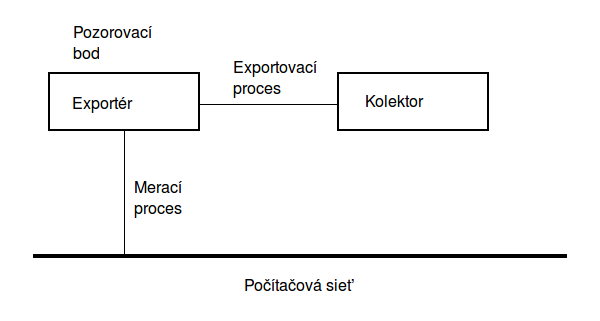
\includegraphics[width=0.7\textwidth]{ipfix_architekture_basic}
\caption{Zjednodušená verzia IPFIX architektúry}\label{o:ipfix_architekture_basic}
\end{figure}

\subsubsection{Terminológia} \label{sec:ipfix_terminology}

Podľa \citep{rfc3917} existuje veľa definícií termínu \uv{tok} používaných Internetovou komunitou.
Pracovná skupina IPFIX používa nasledujúcu:
\begin{description}
  \item[Tok] je definovaný ako množina IP paketov prechádzajúcich pozorovacím bodom v~sieti, počas určitého 
časového intervalu. Všetky pakety patriace príslušnému toku majú množinu spoločných vlastností. Opačne 
môžeme tvrdiť, že každý paket patrí toku, ak spĺňa všetky tieto spoločné vlastnosti. 
\end{description}

Ďalšie termíny zavádza \citep{rfc5101}:
\begin{description}
  \item[Záznam o~toku] obsahuje namerané informácie a charakteristické vlastnosti 
konkrétneho toku, ktorý bol pozorovaný pozorovacím bodom (napr. celkový počet prenesených 
bajtov, zdrojová IP adresa toku, a pod.).

  \item[Pozorovací bod] je miestom v~sieti, kde sú IP pakety pozorované. Medzi príklady patrí 
sieťová linka, na ktorej je zavedená meracia sonda, zdieľané médium (napr. Ethernet LAN), 
alebo fyzické, či logické rozhranie smerovača. Každý pozorovací bod je asociovaný s~
pozorovacou doménou. 

  \item[Pozorovacia doména] je množina pozorovacích bodov. Je identifikovaná číslom 
(Observation Domain ID), ktoré je unikátne v~rámci exportovacieho procesu. 

  \item[Merací proces] vytvára záznamy o~tokoch na základe hlavičiek paketov. Vykonáva 
rôzne funkcie ako napríklad odchytávanie hlavičiek paketov, vytváranie časových známok, 
vzorkovanie, klasifikovanie a údržba záznamov o~tokoch. 

  \item[Exportovací proces] odosiela záznamy o~tokoch zhromažďovacím 
procesom. Tieto záznamy sú generované jedným alebo viacerými meracími procesmi.
	
  \item[Exportér] odosiela dáta o~tokoch. Je to nástroj ktorý zastrešuje exportovacie procesy.

  \item[Kolektor] je nástroj, ktorý prijíma dáta od exportéra. Pozostáva z~jedného, alebo
viacerých zhromažďovacích procesov.

  \item[Zhromažďovací proces] prijíma záznamy o~tokoch od jedného, alebo viacerých 
exportovacích procesov. Prijaté záznamy môže spracovávať, alebo uchovávať. 

  \item[Informačné elementy] sú protokolovo nezávislým popisom atribútov záznamov o~tokoch. 
Informačný model IPFIX \citep{rfc5102} obsahuje základnú množinu informačných elementov, vrátane ich
popisu, významu, dátového typu a pod. Informačné elementy sú rozdelené do 12 skupín, pozri Tabuľku \ref{t:ie-table},
na základe ich sémantiky a použitia. Každý element je asociovaný s~dátovým typom, ktorý určuje jeho 
formát a spôsob kódovania.
Na základe tohto modelu sú jednotlivé dátové záznamy kódované na strane exportéra a dekódované 
v~kolektore.
Informačný model povoľuje aj jeho rozširovanie. Organizácie môžu definovať vlastné informačné
elementy, ktorým musia prideliť unikátny identifikátor. 
Tieto elementy navyše obsahujú identifikátor organizácie \emph{(PEN)}, ktorý musí byť registrovaný v~
IANA\footnote{http://www.iana.org/assignments/enterprise-numbers}.

% ---- tabulka ----
\tabcolsep=8pt
\begin{table}[!ht]\caption{Základné skupiny informačných elementov podľa \citep{rfc5102}}\label{t:ie-table}
\smallskip
\centering
\begin{tabular}{|c|c|}
\hline
\textbf{\#} & \textbf{názov skupiny} \\ \hline
1. & Identifikátory \\ \hline
2. & Konfigurátory meracieho a exportovacieho procesu \\ \hline
3. & Štatistické hodnoty meracieho a exportovacieho procesu \\ \hline
4. & Polia IP hlavičky \\ \hline
5. & Polia transportnej hlavičky \\ \hline
6. & Polia ostatných hlavičiek \\ \hline
7. & Odvodené vlastnosti paketov \\ \hline
8. & Min/Max vlastnosti tokov \\ \hline
9. & Časové známky tokov \\ \hline
10. & Počítadla vlastností tokov \\ \hline
11. & Rôzne vlastnosti tokov \\ \hline
12. & Výplň \emph{(padding)} \\ \hline
\end{tabular}
\end{table}

% -----------

\clearpage
  \item[Šablóna] špecifikuje formát odosielaných záznamov o~tokoch pomocou zoznamu 
informačných elementov. Musí byť odoslaná kolektoru 
z~exportovacieho procesu ešte pred odoslaním samotných dát. Neskôr sú šablóny periodicky 
preposielané, aby kolektor vedel v~každom okamihu aký formát dát prijme. 
Šablóny musia byť dostupné administrátorom, preto sú definované v~konfiguračnom súbore 
exportéra.
\citep{juvhaugen}
\end{description}



\subsubsection{Formát IPFIX správ} \label{sec:message_format}

Formát správ je definovaný v~Špecifikácii IPFIX Protokolu \citep{rfc5101}. Správa pozostáva z~
hlavičky, nasledovaná niekoľkými IPFIX sadami. 
Exportér musí zakódovať všetky časti správy v~sieťovom poradí bajtov (Big-Endian).
Na Obrázku~\ref{o:ipfix_message_format} je jedna z~možností formátu IPFIX správy. Za hlavičkou nasleduje sada šablón, pretože
šablóny musia byť exportované ihneď po vytvorení. Za šablónami nasledujú dátové sady a sady šablón možností 
v~akomkoľvek poradí.

\begin{figure}[ht!]
\centering
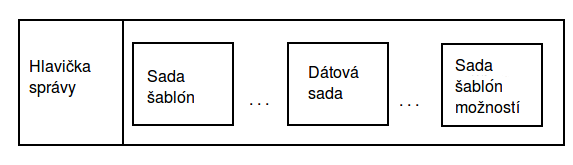
\includegraphics[width=0.7\textwidth]{ipfix_message_format}
\caption{Príklad formátu IPFIX správy}\label{o:ipfix_message_format}
\end{figure}



\paragraph{Formát hlavičky správy}

Formát hlavičky správy je znázornený na~Obrázku~\ref{o:ipfix_message_header}. Pozostáva z~piatich poli:
\begin{itemize}
 \item \textbf{Číslo verzie} záznamu toku v~správe. Pre IPFIX je to hodnota \verb|0x000a|.
 \item \textbf{Dĺžka} predstavuje celkovú dĺžku IPFIX správy v~oktetoch, vrátane hlavičky a sád. 
 \item \textbf{Čas exportu} vo formáte UNIX timestamp. 
 \item \textbf{Sekvenčné číslo} vyjadruje počet odoslaných záznamov dátových záznamov modulo $2^{32}$  
 exportovacím procesom v~tejto transportnej relácii. Túto hodnotu používa kolektor na odhalenie chýbajúcich 
 správ resp. dátových šablón.
 \item \textbf{Identifikačné číslo pozorovacej domény}, ktorý je lokálne jedinečný pre exportovací proces.
 \end{itemize}
 
\begin{figure}[ht!]
\centering
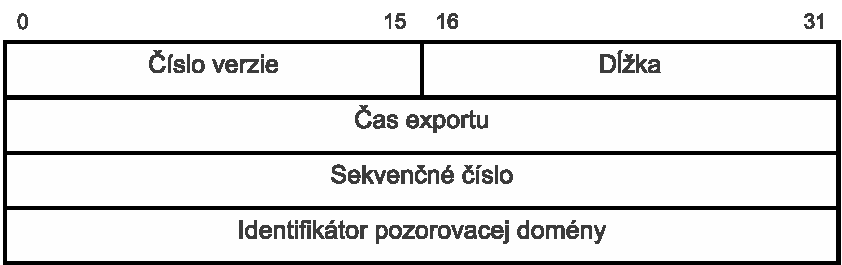
\includegraphics[width=0.7\textwidth]{ipfix_message_header}
\caption{Formát hlavičky IPFIX správy}\label{o:ipfix_message_header}
\end{figure}



\paragraph{Formát sady}

V~IPFIX terminológii je sada všeobecný pojem pre kolekciu záznamov s~podobnou štruktúrou. 
IPFIX správa môže obsahovať tri rôzne druhy sád:
\begin{itemize}
 \item Sada šablón,
 \item Dátová sada,
 \item Sada šablón možností.
\end{itemize}
Každá zo sád sa skladá z~hlavičky sady a jedného, alebo viacerých záznamov sady, Obrázok \ref{o:set_format}. 
Na úplnom konci môže byť vložená výplň \emph{(padding)}, no nie je to povinná súčasť sady. Exportovací proces ho pridáva 
iba v~tom prípade, keď chce aby sada bola zarovnaná na dĺžku, ktorá je násobkom 4, alebo 8.

\begin{figure}[ht!]
\centering
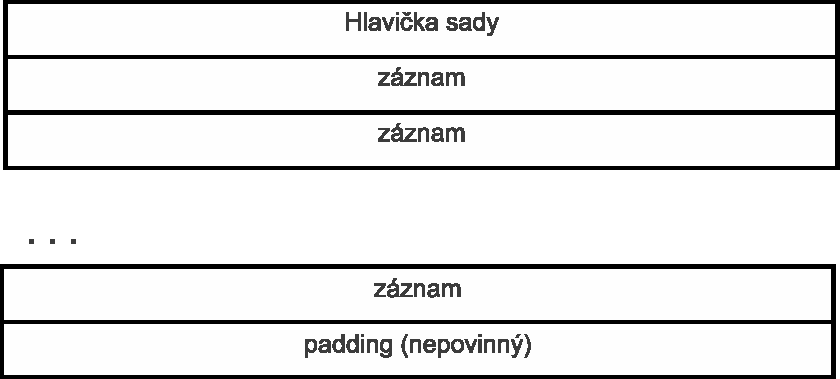
\includegraphics[width=0.7\textwidth]{set_format}
\caption{Formát sady}\label{o:set_format}
\end{figure}

\textbf{Hlavička sady} je rovnaká pre všetky tri typy sád. Je zobrazená na Obrázku \ref{o:set_header}. 
\emph{Identifikátor sady} určuje typ sady a teda aj typ všetkých záznamov obsiahnutých v~sade, pozri 
Tabuľku \ref{t:set-record}. 
Sada istého druhu nemôže obsahovať záznamy iného typu. 
Hodnota 2 je rezervovaná pre sadu šablón. Sada šablón možností nadobúda 
hodnotu 3. Identifikátory 0 a 1 sa nepoužívajú z~historických dôvodov \citep{rfc3954} a hodnoty od 4 po 
255 sú rezervované pre budúce použitie. Dátové sady sú označené hodnotami väčšími ako 255. 


\begin{figure}[ht!]
\centering
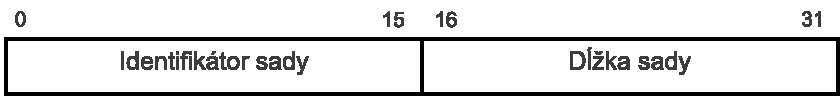
\includegraphics[width=0.7\textwidth]{set_header}
\caption{Formát hlavičky sady}\label{o:set_header}
\end{figure}

\emph{Dĺžka sady} zahŕňa celkovú dĺžku všetkých sád, vrátane hlavičky sady a prípadne výplne. Na jej základe 
sa určuje koniec tejto sady a začiatok ďalšej, pretože sada môže obsahovať rôzny počet záznamov.

% ---- tabuľka ----
\tabcolsep=8pt
\begin{table}[!ht]\caption{Prehľad identifikátorov, typov a záznamov sady}\label{t:set-record}
\smallskip
\centering
\begin{tabular}{|c|c|c|}
\hline
\textbf{Identifikátor sady} & \textbf{typ sady} & \textbf{typ záznamov} \\ \hline
0 - 1 & -- & -- \\ \hline
2 & sada šablón & záznamy šablóny \\ \hline
3 & sada šablón možností & záznamy šablóny možností \\ \hline
4 - 255 & -- & -- \\ \hline
255 - 65535 & dátová sada & dátové záznamy \\ \hline
\end{tabular}
\end{table}
% -----------


\paragraph{Špecifikátory poľa}

Špecifikátor poľa je akousi obálkou nad informačným elementom (Obrázok~\ref{o:field_specifier_format}) -- 
vďaka nemu vie zhromažďovací proces spracovávať prijaté dáta. 

Prvý bit sa nazýva \emph{Enterprise bit}.
Ak je nastavený na 0, tak hovoríme o~oficiálnom informačnom elemente charakterizovanom organizáciou IETF a 
registrovanom v~IANA. 
V~tomto prípade je \emph{číslo organizácie (PEN)} nevyplnené. V~opačnom prípade, 
keď je tento bit nastavený na 1, ide o~organizáciou špecifikovaný informačný element a číslo organizácie
musí byť zadané. Laboratórium počítačových sietí na Technickej univerzite v~Košiciach má pridelené číslo 
organizácie 26235 \citep{pen}.
Dĺžka poľa vyjadruje na koľkých oktetoch je daný informačný element kódovaný. 
Zoznam informačných elementov aj s~ich dĺžkami je dostupný v~\citep{rfc5102}.
Špeciálny prípad nastáva pri redukovanom kódovaní. Vtedy je dĺžka poľa menšia ako popisuje 
Informačný model. 
 
\begin{figure}[ht!]
\centering
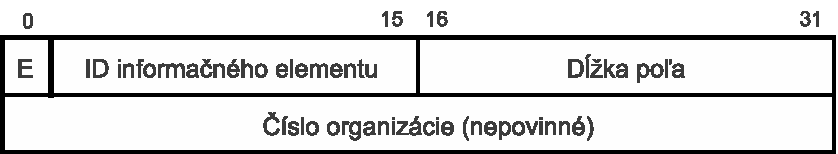
\includegraphics[width=0.7\textwidth]{field_specifier_format}
\caption{Formát špecifikátora poľa}\label{o:field_specifier_format}
\end{figure}



\paragraph{Formát záznamov šablóny}

Záznamy šablóny patria k~nevyhnutným prvkom IPFIX správy. Na ich základe, a základe Informačného modelu
IPFIX \citep{rfc5102} vie zhromažďovací proces dekódovať dátové záznamy.
Šablóny môžu obsahovať akúkoľvek kombináciu informačných elementov. Či už oficiálnych -- navrhnutých 
spoločnosťou IANA, alebo vlastných -- vytvorených organizáciami.

Záznam šablóny tvorí \emph{hlavička}, pozri Obrázok \ref{o:template_record_header}, nasledovaná 
\emph{špecifikátormi poľa}. 
Každá šablóna musí mať v~rámci transportnej relácie a pozorovacej domény jedinečný \emph{identifikátor}. 
Čísluje sa od 255 do 65535, rovnako ako identifikátory dátových sád, pretože každá šablóna referuje 
na dátovú sadu, ktorej štruktúru popisuje. \emph{Počet polí} sa týka počtu 
špecifikátorov poľa.

\begin{figure}[ht!]
\centering
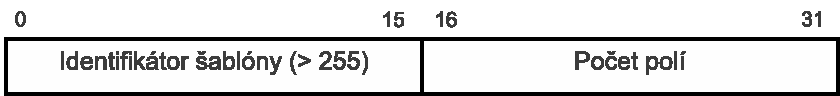
\includegraphics[width=0.7\textwidth]{template_record_header}
\caption{Formát hlavičky záznamu šablóny}\label{o:template_record_header}
\end{figure}



\paragraph{Formát záznamov šablóny možností}

Tieto záznamy dávajú exportéru možnosť poskytnúť kolektoru dodatočné informácie o~kontexte posielaných dát, 
ktoré by zo samotných 
záznamov tokov nevedel vyčítať. Príkladom týchto informácií sú kľúče tokov, alebo konfigurácia šablóny,
vzorkovacie parametre a pod.

Formát záznamov (Obrázok~\ref{o:options_record_header}) je podobný ako v~prípade záznamov šablóny. Pozostáva z~hlavičky záznamu 
a jedného, alebo viacerých špecifikátorov poľa. Formát špecifikátorov je rovnaký ako pri záznamoch šablóny.
Hlavička naviac obsahuje \emph{počet polí pôsobnosti}. Pôsobnosť charakterizuje kontext 
informácií. Šablóna povoľuje 
definovať viac polí pôsobnosti ako jedno. V~tomto prípade je celková pôsobnosť daná kombináciou týchto polí.
Počet polí pôsobnosti nemôže byť nulový, pričom \emph{počet polí} je 
súčtom polí pôsobnosti a špecifikátorov poľa.\citep{rfc5102}

\begin{figure}[ht!]
\centering
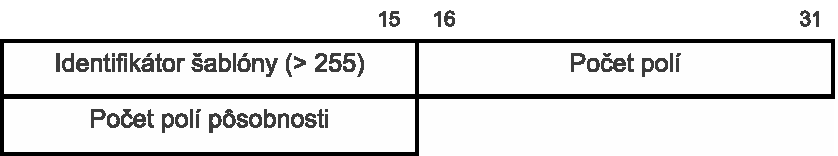
\includegraphics[width=0.7\textwidth]{options_record_header}
\caption{Formát hlavičky záznamu šablóny možností}\label{o:options_record_header}
\end{figure}



\paragraph{Formát dátových záznamov}

Dátové záznamy sú posielané v~dátových sadách. Ich formát je veľmi 
jednoduchý. Pozostávajú len z~hodnôt polí, nemajú ani vlastnú hlavičku. 
Sú kódované podľa popisu v~Informačnom modeli \citep{rfc5102}. Identifikátor 
šablóny, ktorá popisuje tieto hodnoty je zakódovaný v~hlavičke sady, v~časti
identifikátor sady. Inými slovami \uv{identifikátor sady} = \uv{identifikátor 
šablóny}. Aby vedel kolektor tieto dáta dekódovať, musí poznať formát šablóny 
už pred prijatím prvého dátového záznamu.

\subsection{Anal\'yza sprostredkovania spr\'av v IPFIX}

Výhodou monitorovania sieťovej prevádzky na báze tokov je to, že je možné merať 
veľké množstvo sieťovej prevádzky v distribuovaných pozorovacích bodoch. 
Zatiaľ čo tento typ monitorovania môže byť použitý na rôzne účely a pre rozmanité aplikácie, je veľmi 
obtiažne aplikovať ho paralelne na viac aplikácii s veľmi rozdielnymi požiadavkami.
Sieťoví administrátori musia nastaviť parametre meracích nástrojov tak, aby vyhoveli požiadavkám každej
jednej monitorovacej aplikácii. Takéto konfigurácie často nie sú podporované meracími nástrojmi. Či už
kvôli funkčným obmedzeniam, alebo kvôli pamäťovým a výpočtovým limitom, ktoré zamedzujú meraniu veľkých 
dátových tokov. Sprostredkovanie správ v IPFIX - \emph{IP Flow Information Export (IPFIX) Mediation}
vypĺňa túto medzeru medzi obmedzenými možnosťami merania a požiadavkami na monitorovacie aplikácie 
zavedením sprostredkovateľského zariadenia nazývaného \emph{IPFIX Mediátor} \citep{rfc5982}.

\subsubsection{Terminológia}
Terminológia použitá v tejto kapitole je čiastočne definovaná v podkapitole \ref{sec:ipfix_terminology} 
na strane \pageref{sec:ipfix_terminology}. 
Dodatočne zadefinujeme nasledujúce termíny:
\begin{description}
 \item[Prúd záznamov] - \emph{record stream} je sled dát nesúcich informácie o tokoch.
 
 \item[Sprostredkovanie správ v IPFIX] - \emph{IPFIX Mediation} je manipulácia a konverzia prúdu záznamov
 pomocou IPFIX protokolu.
 
 \item[Sprostredkovateľský proces] - \emph{Intermediate Process} prijíma prúd záznamov ako vstupnú 
 veličinu od zhromažďovacieho procesu, meracieho procesu, čítačky IPFIX súborov, iného 
 sprostredkovateľského zariadenia, alebo akéhokoľvek zdroja záznamov. Nad prijatými záznamami
 vykoná rôzne transformácie, na základe ich obsahu. Napokon zmenené záznamy posúva na svoj výstup buď
 smerom k exportovaciemu procesu, inému sprostredkovateľskému zariadeniu, alebo zapisovaču IPFIX súborov
 za účelom vykonania sprostredkovania IPFIX správ.
 
 \item[IPFIX Mediátor] je nástroj vykonávajúci sprostredkovanie správ tak, že prijíma prúd záznamov 
 z rôznych dátových zdrojov, zastrešuje jeden alebo viac sprostredkovateľských procesov  
 aby modifikoval obsah prúdu a nakoniec exportuje pozmenené dáta vo forme IPFIX správ pomocou exportovacieho
 procesu. V typickom prípade prijíma Mediátor prúd záznamov od zhromažďovacieho procesu. No rovnako môže
 prijímať údaje od iných zdrojov, ktoré nie sú zakódované pomocou IPFIX, napr. v prípade konverzie 
 protokolu NetFlow verzie 9 \citep{rfc3954} na IPFIX. Príklad jednej z možných architektúr, 
 v ktorej je použitý Mediátor je na obrázku \ref{o:exp_med_coll} \citep{rfc5982}.
\end{description}

\begin{figure}[ht!]
\centering
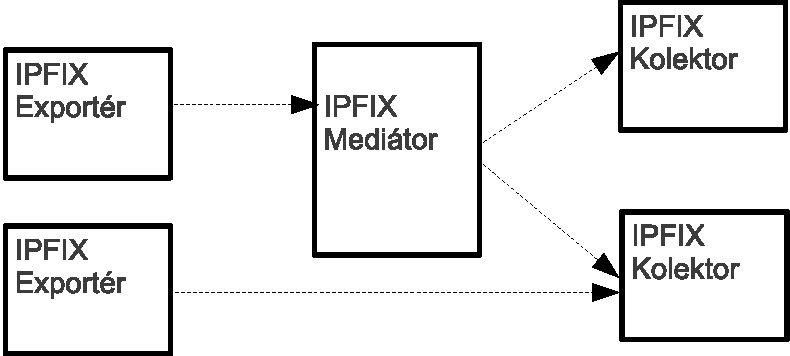
\includegraphics[width=0.7\textwidth]{exp_med_coll}
\caption{Príklad jednej z možných architektúr exportér - mediátor - kolektor}\label{o:exp_med_coll}
\end{figure}



\subsubsection{Anal\'yza nev\'yhod architekt\'ury bez Medi\'atora}


Problematika sprostredkovania IPFIX správ je podrobne spracovaná v \citep{rfc5982}. 
Hovori o tom, že sieťoví administrátori často celia problémom týkajúcim sa škálovateľnosti meracieho 
systému, flexibility monitorovania na základe tokov, alebo aj spoľahlivosti exportovania.
Napriek tomu, že sa vyvinuli známe techniky ako \emph{vzorkovanie a filtrovanie  paketov}, \emph{zoskupovanie 
dátových záznamov}, alebo \emph{replikácia exportu}, tieto problémy nevymizli.
Pozostávajú z prispôsobovania niektorých parametrov meracích nástrojov zdrojom meracieho 
systému zatiaľ čo musia naplniť patričné podmienky ako sú \emph{presnosť nameraných dát}, \emph{granularita 
toku}, či \emph{spoľahlivosť exportu}. Tieto okolnosti závisia na dvoch faktoroch:
\begin{enumerate}
 \item \textbf{Kapacita  meracieho systému} - pozostáva zo šírky pásma  spravovanej siete, kapacity 
 úložiska a výkonu exportovacích a zhromažďovacích nástrojov
 
 \item \textbf{Požiadavky aplikácie} - rôzne aplikácie vyžadujú rôznu zrnitosť záznamov o tokoch a presnosť dát.
\end{enumerate}



\paragraph{Vyrovnanie sa s rastom sieťovej prev\'adzky}

Veľké spoločnosti a poskytovatelia Internetového pripojenia (ISP) majú bežne vo svojej sieťovej 
infraštruktúre linky so šírkou pásma 10 Gb/s a ich celková sieťová prevádzka presahuje 100 Gb/s. 
Podla \citep{trafgrw} sieťová prevádzka používateľov širokopásmového pripojenia k
Internetu v blízkej budúcnosti sa bude každým rokom zvyšovať približne o 40\%. Sieťoví administrátori
monitorujúci IP prevádzku môžu udržiavať krok s týmto nárastom vďaka použitiu viacerých exportérov. 
Tento prístup však môže viesť k prekročeniu výpočtových a pamäťových možností jediného kolektora.

Tento problém zmierňujú redukčné techniky \emph{vzorkovanie a filtrovanie paketov} popísané v \citep{rfc5475}
implementované v exportéroch. Podobne agregácia meraných dát. Tieto techniky však majú aj svoje nevýhody. 
Môžu viesť k stratám malých tokov, nemožnosti odhalenia drobných zmien a anomálií v prenášaných dátach. 
Filtrovanie spôsobuje, že len podmnožina dátových záznamov je exportovaná.

Vzhľadom k týmto nedostatkom sa vyžaduje aby sa veľké meracie infraštruktúry nespoliehali na 
spomínané redukčné techniky.


\paragraph{Vyrovnanie sa s viacúčelovým meraním}

Rôzne monitorovacie aplikácie majú rôzne požiadavky na meraciu infraštruktúru. Niektoré vyžadujú 
monitorovanie na úrovni tokov, iné informácie o individuálnych paketoch a ďalšie agregované toky a pod.

Ak by mal exportér naplniť tieto požiadavky, musel by paralelne vykonávať rôzne meracie operácie, čo je
kvôli limitovaným výpočtovým zdrojom takmer nemožné. Preto je výhodnejšie použiť exportér s jednoduchším a 
výkonnejším nastavením a namerané dáta vhodne spracovávať na ďalšej úrovni meracej architektúry.



\paragraph{Vyrovnanie sa s heterogénnym prostredím}

Administrátori môžu použivať IPFIX nástroje od rozmanitých výrobcov, s rozdielnymi verziami softvéru a s 
rôznymi typmi sieťových zariadení (smerovač, prepínač, meracia sonda) v jednej sieťovej doméne.
V niektorých topológiách sú stále nasadené historické protokoly na export tokov. Dosiahnutie plnej 
interoperability týchto zariadení nie je možné.

Monitorovací systém sa vie vysporiadať s týmto problémom iba keď je prítomné sprostredkovanie IPFIX správ.
Avšak obsiahnuť sprostredkovanie vo všetkých zhromažďovacích zariadeniach je náročné.


\paragraph{Zhrnutie problémov}

Vzhľadom k limitovaným zdrojom monitorovacieho systému, je dôležité použiť techniky redukcie sieťových 
dát čím nižšie v hierarchii systému, teda v exportéri. Avšak implementácia tohto návrhu je sťažená v 
heterogénnom prostredí exportovacích nástrojov. 
Na druhej strane, udržovanie presnosti dát a granularity tokov tak, aby boli splnené požiadavky 
rôznych monitorovacích aplikácii vyžaduje škálovateľnú a flexibilnú zhromažďovaciu infraštruktúru.

Toto zhrnutie implikuje, že nové sprostredkovateľské funkcie sú potrebné v typických exportér - kolektor
infraštruktúrach. 


\subsubsection{Vybrané príklady použitia sprostredkovania správ} \label{sec:mediator_examples}


RFC 5982 \citep{rfc5982} uvádza viacero príkladov zaradenia IPFIX Mediátora do klasickej
exportér - kolektor architektúry. Uveďme aspoň niektoré.


\paragraph{Prispôsobovanie granularity tokov}

Najzákladnejšia sada kľúčov toku je pätica: \emph{protokol}, \emph{zdrojová a cieľová IP adresa}, 
\emph{číslo zdrojového a cieľového portu}. Menšie sady kľúčov, teda trojice, dvojice, alebo len jeden 
samotný prvok (napr. \emph{maska siete}, \emph{BGP čísla autonómnych systémov}, a pod.) vytvárajú viac 
agregované záznamy o tokoch. Toto je vhodné pri meraní na úrovni 
jadra sieťovej domény, alebo pri manipulovaní s výkonnosťou exportérov a kolektorov.

Najvhodnejšia implementácia predstavuje konfigurovateľný merací proces v exportéri. Administrátor 
špecifikuje požadovanú sadu kľúčov toku a tým pádom exportér generuje záznamy o toku želanej zrnitosti.

V opačnom prípade, kde merací proces nemá schopnosť nastavovať kľúče toku exportéra, IPFIX Mediátor 
môže agregovať dátové záznamy na základe definovaných kľúčov vo svojej konfigurácii.


\paragraph{Distribuovaná zhromažďovacia infraštruktúra}

Zvyšovanie počtu IPFIX exportérov, rast objemu IP dát a rôzne požiadavky na operácie vykonávané nad 
dátovými záznamami v kolektore spôsobujú vysokú náročnosť na implementáciu všetkých meracích
aplikácii v rámci jedného kolektora.

Za účelom navýšenia zhromažďovacej kapacity resp. objemu spracovania dátových záznamov musia byť 
nasadené distribuované kolektory čím bližšie ku exportérom. V tomto prípade sa kolektory stanú 
IPFIX Mediátormi, ktoré budú preposielať dátové záznamy podľa požiadaviek centralizovaným aplikáciam.


\paragraph{Spájanie času}

Spájanie resp. kompozícia času je definovaná ako agregácia za sebou idúcich dátových záznamov s rovnakými
kľúčmi toku. Tento proces vedie k rovnakému výstupu ako nastavenie dlhšieho aktívneho timeoutu
\emph{(active timeout)} v exportéri, no má jednu výhodu. Nové metriky ako napríklad výpočet priemerných, 
maximálnych, alebo minimálnych hodnôt zo záznamov o tokoch v kratších časových intervaloch umožňujú 
presnejšie výsledky a sledovanie aj menších zmien.

Jedna z možných implementácii je použitie sprostredkovateľského procesu umiestneného medzi 
meracím a exportovacím procesom exportéra. Druhou možnosťou je samostatný IPFIX Mediátor situovaný medzi
exportérom a kolektorom. Táto možnosť prináša väčšiu flexibilitu a nezaťažuje exportér ďalšími výpočtami.


\paragraph{Spájanie priestoru} \label{sec:spatial}

Spájanie priestoru je vlastne zoskupenie dátových záznamov v rámci množiny pozorovacích bodov jednej 
pozorovacej domény, združovanie záznamov viacerých exportérov, alebo jedného exportéra ale viacerých 
pozorovacích domén. Delí sa na tieto štyri typy:

\begin{enumerate}
 \item \textbf{Spájanie priestoru v rámci jednej pozorovacej domény} \\ 
    Príkladom je meranie dátového toku jedného logického rozhrania, ktoré vzniklo agregáciou liniek 
    podla 802.3ad \citep{ieee802.3}.
 \item \textbf{Spájanie priestoru viacerých pozorovacích domén jedného exportéra} \\
    Tak isto ako v predchádzajúcom príklade aj tu ide o agregáciu viacerých fyzických liniek. 
 \item \textbf{Spájanie priestoru niekoľkých exportérov} \\
    Dátové záznamy namerané v rámci jednej administratívnej domény môžu byť zlučované.
 \item \textbf{Spájanie priestoru administratívnych domén} \\
    Dátové záznamy zaznamenané vo viacerých administratívnych doménach, ako napríklad v rôznych klientskych 
    sieťach, alebo v sieťach rozdielnych poskytovateľov Internetového pripojenia môžu byť tiež zlučované.
    Kolektor vie na základe IP adresy exportéra rozlíšiť, ktorej klientskej sieti exportér patrí a tak 
    rozlišovať klientske dáta.
\end{enumerate}

Implementácia pomocou sprostredkovateľského procesu umiestneného v exportéri rieši prípady 1 a 2. 
Separátny IPFIX Mediátor je riešením pre  všetky štyri prípady.


\paragraph{Anonymizácia dátových záznamov}

IPFIX exporty krížom cez administratívne domény, tak ako to bolo popísané v prípade 4 
v podkapitole \ref{sec:spatial}, na strane \pageref{sec:spatial} môžu 
byt použité na monitorovanie sieťovej prevádzky na veľké vzdialenosti, 
napríklad pre analýzu dátových trendov v Internete. Pri takomto použití sa musia administrátori riadiť
pravidlami pre ochranu súkromia a predísť monitorovaniu dôvernej sieťovej prevádzky cudzími osobami.
Typicky anonymizačné techniky umožňujú poskytovanie sieťových dát iným osobám bez porušenia týchto zásad.

Všeobecne platí, že anonymizácia upraví sadu dát tak, aby chránila identitu ľudí alebo subjektov, 
ktorých sa súbor dát týka. Zároveň sa pokúša zachovať dáta tak, aby boli stále zmysluplné pre danú 
analýzu ale súčasne nemôžu byť stopovateľné naspäť ku konkrétnym sieťam, pracovným staniciam, alebo 
používateľom generujúcim tieto dáta. Napríklad, anonymizácia IP adresy je veľmi dôležitá pre 
zamedzenie identifikácie užívateľov, alebo smerovačov. 

Jedným z možných prevedení v tomto prípade používa anonymizačnú funkciu v exportéri. 
To však príliš zvyšuje zaťaženie exportéra. Flexibilnejšia implementácia využíva samostatný 
IPFIX Mediátor medzi exportérom a kolektorom.


\paragraph{Distribúcia dátových záznamov}

Trendom v moderných dátových sieťach je súčasný prenos dát, hlasu a video komunikácie jednou 
spoločnou infraštruktúrou. Takéto siete nazývame konvergovanými sieťami. 
Počítačové siete paralelne prenášajú dáta viacerých protokolov ako napríklad
IPv4, IPv6, VPN, MPLS a pod. Dátové záznamy každého z týchto protokolov musia byť analyzované 
oddelene a z rôznych perspektív pre rôzne organizácie.

Jeden kolektor pokrývajúci všetky typy dátových záznamov sa môže stať úzkym hrdlom 
zhromažďovacej infraštruktúry. Preto je lepšie distribuovať dátové záznamy na základe ich 
typu viacerým kolektorom, čo má za následok rozloženie zátaže. Pod typom dátového 
záznamu máme na mysli napríklad typ sieťového protokolu, ktorým boli dáta prenášane. 

Jedna z možných implementácií v tomto prípade používa replikáciu IPFIX správy v exportéri 
pre viac kolektorov. Každý kolektor potom dekóduje tie dátové záznamy, ktoré jeho aplikácia
potrebuje. To však zvyšuje zaťaženie exportovacieho procesu a mrhanie šírkou pásma medzi
exportérom a kolektorom.

Sofistikovanejšie prevedenie používa sprostredkovateľský proces v exportéri, ktorý určuje, 
ktorému kolektoru sa dáta pošlú, v závislosti na hodnotách určitých polí. Ak exportér nemá
túto schopnosť, posiela dátové záznamy IPFIX Mediátoru, a ten ich distribuuje kolektorom.


\paragraph{Interoperabilita medzi protokolmi starších verzií a IPFIX}

Počas migrácie z protokolov starších verzií ako napríklad NetFlow \citep{rfc3954} na IPFIX
zvyknú nástroje týchto protokolov súčasne existovať v jednej sieti. Napríklad aj po zavedení 
IPFIX kolektora je nutné monitorovať sieť, hoci exportér je verzie NetFlow.

Jedna z možností je použiť IPFIX Mediátor, ktorý bude konvertovať starší protokol na IPFIX.



\subsubsection{Vybrané implementačno-špecifické problémy IPFIX Mediátora} \label{sec:problems}


\paragraph{Strata informácie o pôvodnom exportéri} \label{sec:loss_info}

Pri využívaní sprostredkovania správ v IPFIX dochádza k strate potrebných informácii. V prvom rade to je 
IP adresa exportéra, ktorá bola získavaná zo zdrojovej IP adresy transportnej relácie, rovnako 
ako identifikačné číslo pozorovacej domény, ktoré je zahrnuté v hlavičke IPFIX správy.
V niektorých prípadoch môže Mediátor zahodiť tieto informácie úmyselne. 
Vo všeobecnosti však platí, že kolektor musí rozpoznať pôvod nameraných dát, ako napríklad IP adresu 
exportéra, ID pozorovacej domény, alebo dokonca ID pozorovacieho bodu. Ak Mediátor tieto informácie 
o exportéri neoznámi kolektoru, tak ten nesprávne usúdi, že IP adresa Mediátora je adresa pôvodcu dát 
(exportéra).

V nasledujúcom obrázku \ref{o:loss_of_exporter} kolektor vie rozoznať dve IP adresy - 192.0.2.3. (Mediátor) 
a 192.0.2.2 (exportér 2). To nie je správne. Mediátor musí informovať kolektor o IP adrese exportéra 1.

\begin{figure}[ht!]
\centering
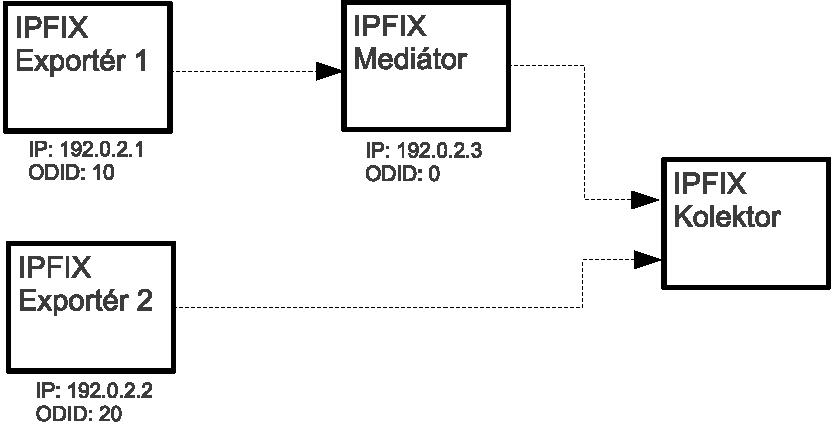
\includegraphics[width=0.7\textwidth]{loss_of_exporter}
\caption{Strata informácie o originálnom exportéri}\label{o:loss_of_exporter}
\end{figure}


\paragraph{Strata informácie o čase exportu} \label{sec:loss_time}

Pole čas exportu \emph{export time}, ktoré je zahrnuté v hlavičke správy predstavuje referenčnú 
časovú známku dátové záznamy. Niektoré informačné elementy popísané v \citep{rfc5102} nesú 
časové známky delta \emph{delta timestamps}, ktoré udávajú časový rozdiel voči hodnote v poli 
čas exportu. Ak dátový záznam zahŕňa nejaké pole s časovou známkou delta a Mediátor prepíše hodnotu 
času exportu,  tak časová známka delta týmto stráca význam. Kolektor však túto situáciu nevie 
rozpoznať a tak pracuje so zlými hodnotami.


\paragraph{Interpretácia sprostredkovaných správ}

V niektorých prípadoch potrebuje kolektor vedieť, ktoré konkrétne operácie resp. funkcie vykonal Mediátor 
nad dátovými záznamami. Kolektor nedokáže rozlíšiť medzi spájaním času a spájaním priestoru, v prípade, že 
Mediátor neexportuje použitú funkciu. Niektoré parametre vzťahujúce sa k funkcii by tiež mali byť 
exportované. 

V prípade spájania času, kolektor musí poznať aktívny timeout \emph{active timeout} 
pôvodných záznamov o tokoch. Pri spájaní priestoru je potrebné poznať nad akou oblasťou bola 
vykonaná kompozícia dátových záznamov.\citep{rfc5982}



%
\subsection{Anal\'yza sprostredkovania spr\'av v IPFIX}

Výhodou monitorovania sieťovej prevádzky na báze tokov je to, že je možné merať 
veľké množstvo sieťovej prevádzky v distribuovaných pozorovacích bodoch. 
Zatiaľ čo tento typ monitorovania môže byť použitý na rôzne účely a pre rozmanité aplikácie, je veľmi 
obtiažne aplikovať ho paralelne na viac aplikácii s veľmi rozdielnymi požiadavkami.
Sieťoví administrátori musia nastaviť parametre meracích nástrojov tak, aby vyhoveli požiadavkám každej
jednej monitorovacej aplikácii. Takéto konfigurácie často nie sú podporované meracími nástrojmi. Či už
kvôli funkčným obmedzeniam, alebo kvôli pamäťovým a výpočtovým limitom, ktoré zamedzujú meraniu veľkých 
dátových tokov. Sprostredkovanie správ v IPFIX - \emph{IP Flow Information Export (IPFIX) Mediation}
vypĺňa túto medzeru medzi obmedzenými možnosťami merania a požiadavkami na monitorovacie aplikácie 
zavedením sprostredkovateľského zariadenia nazývaného \emph{IPFIX Mediátor} \citep{rfc5982}.

\subsubsection{Terminológia}
Terminológia použitá v tejto kapitole je čiastočne definovaná v podkapitole \ref{sec:ipfix_terminology} 
na strane \pageref{sec:ipfix_terminology}. 
Dodatočne zadefinujeme nasledujúce termíny:
\begin{description}
 \item[Prúd záznamov] - \emph{record stream} je sled dát nesúcich informácie o tokoch.
 
 \item[Sprostredkovanie správ v IPFIX] - \emph{IPFIX Mediation} je manipulácia a konverzia prúdu záznamov
 pomocou IPFIX protokolu.
 
 \item[Sprostredkovateľský proces] - \emph{Intermediate Process} prijíma prúd záznamov ako vstupnú 
 veličinu od zhromažďovacieho procesu, meracieho procesu, čítačky IPFIX súborov, iného 
 sprostredkovateľského zariadenia, alebo akéhokoľvek zdroja záznamov. Nad prijatými záznamami
 vykoná rôzne transformácie, na základe ich obsahu. Napokon zmenené záznamy posúva na svoj výstup buď
 smerom k exportovaciemu procesu, inému sprostredkovateľskému zariadeniu, alebo zapisovaču IPFIX súborov
 za účelom vykonania sprostredkovania IPFIX správ.
 
 \item[IPFIX Mediátor] je nástroj vykonávajúci sprostredkovanie správ tak, že prijíma prúd záznamov 
 z rôznych dátových zdrojov, zastrešuje jeden alebo viac sprostredkovateľských procesov  
 aby modifikoval obsah prúdu a nakoniec exportuje pozmenené dáta vo forme IPFIX správ pomocou exportovacieho
 procesu. V typickom prípade prijíma Mediátor prúd záznamov od zhromažďovacieho procesu. No rovnako môže
 prijímať údaje od iných zdrojov, ktoré nie sú zakódované pomocou IPFIX, napr. v prípade konverzie 
 protokolu NetFlow verzie 9 \citep{rfc3954} na IPFIX. Príklad jednej z možných architektúr, 
 v ktorej je použitý Mediátor je na obrázku \ref{o:exp_med_coll} \citep{rfc5982}.
\end{description}

\begin{figure}[ht!]
\centering
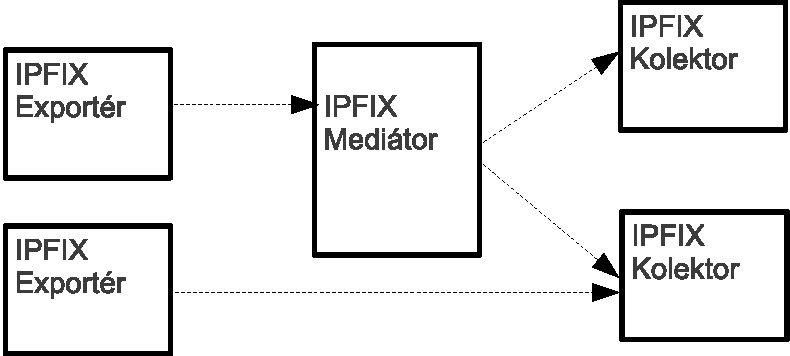
\includegraphics[width=0.7\textwidth]{exp_med_coll}
\caption{Príklad jednej z možných architektúr exportér - mediátor - kolektor}\label{o:exp_med_coll}
\end{figure}



\subsubsection{Anal\'yza nev\'yhod architekt\'ury bez Medi\'atora}


Problematika sprostredkovania IPFIX správ je podrobne spracovaná v \citep{rfc5982}. 
Hovori o tom, že sieťoví administrátori často celia problémom týkajúcim sa škálovateľnosti meracieho 
systému, flexibility monitorovania na základe tokov, alebo aj spoľahlivosti exportovania.
Napriek tomu, že sa vyvinuli známe techniky ako \emph{vzorkovanie a filtrovanie  paketov}, \emph{zoskupovanie 
dátových záznamov}, alebo \emph{replikácia exportu}, tieto problémy nevymizli.
Pozostávajú z prispôsobovania niektorých parametrov meracích nástrojov zdrojom meracieho 
systému zatiaľ čo musia naplniť patričné podmienky ako sú \emph{presnosť nameraných dát}, \emph{granularita 
toku}, či \emph{spoľahlivosť exportu}. Tieto okolnosti závisia na dvoch faktoroch:
\begin{enumerate}
 \item \textbf{Kapacita  meracieho systému} - pozostáva zo šírky pásma  spravovanej siete, kapacity 
 úložiska a výkonu exportovacích a zhromažďovacích nástrojov
 
 \item \textbf{Požiadavky aplikácie} - rôzne aplikácie vyžadujú rôznu zrnitosť záznamov o tokoch a presnosť dát.
\end{enumerate}



\paragraph{Vyrovnanie sa s rastom sieťovej prev\'adzky}

Veľké spoločnosti a poskytovatelia Internetového pripojenia (ISP) majú bežne vo svojej sieťovej 
infraštruktúre linky so šírkou pásma 10 Gb/s a ich celková sieťová prevádzka presahuje 100 Gb/s. 
Podla \citep{trafgrw} sieťová prevádzka používateľov širokopásmového pripojenia k
Internetu v blízkej budúcnosti sa bude každým rokom zvyšovať približne o 40\%. Sieťoví administrátori
monitorujúci IP prevádzku môžu udržiavať krok s týmto nárastom vďaka použitiu viacerých exportérov. 
Tento prístup však môže viesť k prekročeniu výpočtových a pamäťových možností jediného kolektora.

Tento problém zmierňujú redukčné techniky \emph{vzorkovanie a filtrovanie paketov} popísané v \citep{rfc5475}
implementované v exportéroch. Podobne agregácia meraných dát. Tieto techniky však majú aj svoje nevýhody. 
Môžu viesť k stratám malých tokov, nemožnosti odhalenia drobných zmien a anomálií v prenášaných dátach. 
Filtrovanie spôsobuje, že len podmnožina dátových záznamov je exportovaná.

Vzhľadom k týmto nedostatkom sa vyžaduje aby sa veľké meracie infraštruktúry nespoliehali na 
spomínané redukčné techniky.


\paragraph{Vyrovnanie sa s viacúčelovým meraním}

Rôzne monitorovacie aplikácie majú rôzne požiadavky na meraciu infraštruktúru. Niektoré vyžadujú 
monitorovanie na úrovni tokov, iné informácie o individuálnych paketoch a ďalšie agregované toky a pod.

Ak by mal exportér naplniť tieto požiadavky, musel by paralelne vykonávať rôzne meracie operácie, čo je
kvôli limitovaným výpočtovým zdrojom takmer nemožné. Preto je výhodnejšie použiť exportér s jednoduchším a 
výkonnejším nastavením a namerané dáta vhodne spracovávať na ďalšej úrovni meracej architektúry.



\paragraph{Vyrovnanie sa s heterogénnym prostredím}

Administrátori môžu použivať IPFIX nástroje od rozmanitých výrobcov, s rozdielnymi verziami softvéru a s 
rôznymi typmi sieťových zariadení (smerovač, prepínač, meracia sonda) v jednej sieťovej doméne.
V niektorých topológiách sú stále nasadené historické protokoly na export tokov. Dosiahnutie plnej 
interoperability týchto zariadení nie je možné.

Monitorovací systém sa vie vysporiadať s týmto problémom iba keď je prítomné sprostredkovanie IPFIX správ.
Avšak obsiahnuť sprostredkovanie vo všetkých zhromažďovacích zariadeniach je náročné.


\paragraph{Zhrnutie problémov}

Vzhľadom k limitovaným zdrojom monitorovacieho systému, je dôležité použiť techniky redukcie sieťových 
dát čím nižšie v hierarchii systému, teda v exportéri. Avšak implementácia tohto návrhu je sťažená v 
heterogénnom prostredí exportovacích nástrojov. 
Na druhej strane, udržovanie presnosti dát a granularity tokov tak, aby boli splnené požiadavky 
rôznych monitorovacích aplikácii vyžaduje škálovateľnú a flexibilnú zhromažďovaciu infraštruktúru.

Toto zhrnutie implikuje, že nové sprostredkovateľské funkcie sú potrebné v typických exportér - kolektor
infraštruktúrach. 


\subsubsection{Vybrané príklady použitia sprostredkovania správ} \label{sec:mediator_examples}


RFC 5982 \citep{rfc5982} uvádza viacero príkladov zaradenia IPFIX Mediátora do klasickej
exportér - kolektor architektúry. Uveďme aspoň niektoré.


\paragraph{Prispôsobovanie granularity tokov}

Najzákladnejšia sada kľúčov toku je pätica: \emph{protokol}, \emph{zdrojová a cieľová IP adresa}, 
\emph{číslo zdrojového a cieľového portu}. Menšie sady kľúčov, teda trojice, dvojice, alebo len jeden 
samotný prvok (napr. \emph{maska siete}, \emph{BGP čísla autonómnych systémov}, a pod.) vytvárajú viac 
agregované záznamy o tokoch. Toto je vhodné pri meraní na úrovni 
jadra sieťovej domény, alebo pri manipulovaní s výkonnosťou exportérov a kolektorov.

Najvhodnejšia implementácia predstavuje konfigurovateľný merací proces v exportéri. Administrátor 
špecifikuje požadovanú sadu kľúčov toku a tým pádom exportér generuje záznamy o toku želanej zrnitosti.

V opačnom prípade, kde merací proces nemá schopnosť nastavovať kľúče toku exportéra, IPFIX Mediátor 
môže agregovať dátové záznamy na základe definovaných kľúčov vo svojej konfigurácii.


\paragraph{Distribuovaná zhromažďovacia infraštruktúra}

Zvyšovanie počtu IPFIX exportérov, rast objemu IP dát a rôzne požiadavky na operácie vykonávané nad 
dátovými záznamami v kolektore spôsobujú vysokú náročnosť na implementáciu všetkých meracích
aplikácii v rámci jedného kolektora.

Za účelom navýšenia zhromažďovacej kapacity resp. objemu spracovania dátových záznamov musia byť 
nasadené distribuované kolektory čím bližšie ku exportérom. V tomto prípade sa kolektory stanú 
IPFIX Mediátormi, ktoré budú preposielať dátové záznamy podľa požiadaviek centralizovaným aplikáciam.


\paragraph{Spájanie času}

Spájanie resp. kompozícia času je definovaná ako agregácia za sebou idúcich dátových záznamov s rovnakými
kľúčmi toku. Tento proces vedie k rovnakému výstupu ako nastavenie dlhšieho aktívneho timeoutu
\emph{(active timeout)} v exportéri, no má jednu výhodu. Nové metriky ako napríklad výpočet priemerných, 
maximálnych, alebo minimálnych hodnôt zo záznamov o tokoch v kratších časových intervaloch umožňujú 
presnejšie výsledky a sledovanie aj menších zmien.

Jedna z možných implementácii je použitie sprostredkovateľského procesu umiestneného medzi 
meracím a exportovacím procesom exportéra. Druhou možnosťou je samostatný IPFIX Mediátor situovaný medzi
exportérom a kolektorom. Táto možnosť prináša väčšiu flexibilitu a nezaťažuje exportér ďalšími výpočtami.


\paragraph{Spájanie priestoru} \label{sec:spatial}

Spájanie priestoru je vlastne zoskupenie dátových záznamov v rámci množiny pozorovacích bodov jednej 
pozorovacej domény, združovanie záznamov viacerých exportérov, alebo jedného exportéra ale viacerých 
pozorovacích domén. Delí sa na tieto štyri typy:

\begin{enumerate}
 \item \textbf{Spájanie priestoru v rámci jednej pozorovacej domény} \\ 
    Príkladom je meranie dátového toku jedného logického rozhrania, ktoré vzniklo agregáciou liniek 
    podla 802.3ad \citep{ieee802.3}.
 \item \textbf{Spájanie priestoru viacerých pozorovacích domén jedného exportéra} \\
    Tak isto ako v predchádzajúcom príklade aj tu ide o agregáciu viacerých fyzických liniek. 
 \item \textbf{Spájanie priestoru niekoľkých exportérov} \\
    Dátové záznamy namerané v rámci jednej administratívnej domény môžu byť zlučované.
 \item \textbf{Spájanie priestoru administratívnych domén} \\
    Dátové záznamy zaznamenané vo viacerých administratívnych doménach, ako napríklad v rôznych klientskych 
    sieťach, alebo v sieťach rozdielnych poskytovateľov Internetového pripojenia môžu byť tiež zlučované.
    Kolektor vie na základe IP adresy exportéra rozlíšiť, ktorej klientskej sieti exportér patrí a tak 
    rozlišovať klientske dáta.
\end{enumerate}

Implementácia pomocou sprostredkovateľského procesu umiestneného v exportéri rieši prípady 1 a 2. 
Separátny IPFIX Mediátor je riešením pre  všetky štyri prípady.


\paragraph{Anonymizácia dátových záznamov}

IPFIX exporty krížom cez administratívne domény, tak ako to bolo popísané v prípade 4 
v podkapitole \ref{sec:spatial}, na strane \pageref{sec:spatial} môžu 
byt použité na monitorovanie sieťovej prevádzky na veľké vzdialenosti, 
napríklad pre analýzu dátových trendov v Internete. Pri takomto použití sa musia administrátori riadiť
pravidlami pre ochranu súkromia a predísť monitorovaniu dôvernej sieťovej prevádzky cudzími osobami.
Typicky anonymizačné techniky umožňujú poskytovanie sieťových dát iným osobám bez porušenia týchto zásad.

Všeobecne platí, že anonymizácia upraví sadu dát tak, aby chránila identitu ľudí alebo subjektov, 
ktorých sa súbor dát týka. Zároveň sa pokúša zachovať dáta tak, aby boli stále zmysluplné pre danú 
analýzu ale súčasne nemôžu byť stopovateľné naspäť ku konkrétnym sieťam, pracovným staniciam, alebo 
používateľom generujúcim tieto dáta. Napríklad, anonymizácia IP adresy je veľmi dôležitá pre 
zamedzenie identifikácie užívateľov, alebo smerovačov. 

Jedným z možných prevedení v tomto prípade používa anonymizačnú funkciu v exportéri. 
To však príliš zvyšuje zaťaženie exportéra. Flexibilnejšia implementácia využíva samostatný 
IPFIX Mediátor medzi exportérom a kolektorom.


\paragraph{Distribúcia dátových záznamov}

Trendom v moderných dátových sieťach je súčasný prenos dát, hlasu a video komunikácie jednou 
spoločnou infraštruktúrou. Takéto siete nazývame konvergovanými sieťami. 
Počítačové siete paralelne prenášajú dáta viacerých protokolov ako napríklad
IPv4, IPv6, VPN, MPLS a pod. Dátové záznamy každého z týchto protokolov musia byť analyzované 
oddelene a z rôznych perspektív pre rôzne organizácie.

Jeden kolektor pokrývajúci všetky typy dátových záznamov sa môže stať úzkym hrdlom 
zhromažďovacej infraštruktúry. Preto je lepšie distribuovať dátové záznamy na základe ich 
typu viacerým kolektorom, čo má za následok rozloženie zátaže. Pod typom dátového 
záznamu máme na mysli napríklad typ sieťového protokolu, ktorým boli dáta prenášane. 

Jedna z možných implementácií v tomto prípade používa replikáciu IPFIX správy v exportéri 
pre viac kolektorov. Každý kolektor potom dekóduje tie dátové záznamy, ktoré jeho aplikácia
potrebuje. To však zvyšuje zaťaženie exportovacieho procesu a mrhanie šírkou pásma medzi
exportérom a kolektorom.

Sofistikovanejšie prevedenie používa sprostredkovateľský proces v exportéri, ktorý určuje, 
ktorému kolektoru sa dáta pošlú, v závislosti na hodnotách určitých polí. Ak exportér nemá
túto schopnosť, posiela dátové záznamy IPFIX Mediátoru, a ten ich distribuuje kolektorom.


\paragraph{Interoperabilita medzi protokolmi starších verzií a IPFIX}

Počas migrácie z protokolov starších verzií ako napríklad NetFlow \citep{rfc3954} na IPFIX
zvyknú nástroje týchto protokolov súčasne existovať v jednej sieti. Napríklad aj po zavedení 
IPFIX kolektora je nutné monitorovať sieť, hoci exportér je verzie NetFlow.

Jedna z možností je použiť IPFIX Mediátor, ktorý bude konvertovať starší protokol na IPFIX.



\subsubsection{Vybrané implementačno-špecifické problémy IPFIX Mediátora} \label{sec:problems}


\paragraph{Strata informácie o pôvodnom exportéri} \label{sec:loss_info}

Pri využívaní sprostredkovania správ v IPFIX dochádza k strate potrebných informácii. V prvom rade to je 
IP adresa exportéra, ktorá bola získavaná zo zdrojovej IP adresy transportnej relácie, rovnako 
ako identifikačné číslo pozorovacej domény, ktoré je zahrnuté v hlavičke IPFIX správy.
V niektorých prípadoch môže Mediátor zahodiť tieto informácie úmyselne. 
Vo všeobecnosti však platí, že kolektor musí rozpoznať pôvod nameraných dát, ako napríklad IP adresu 
exportéra, ID pozorovacej domény, alebo dokonca ID pozorovacieho bodu. Ak Mediátor tieto informácie 
o exportéri neoznámi kolektoru, tak ten nesprávne usúdi, že IP adresa Mediátora je adresa pôvodcu dát 
(exportéra).

V nasledujúcom obrázku \ref{o:loss_of_exporter} kolektor vie rozoznať dve IP adresy - 192.0.2.3. (Mediátor) 
a 192.0.2.2 (exportér 2). To nie je správne. Mediátor musí informovať kolektor o IP adrese exportéra 1.

\begin{figure}[ht!]
\centering
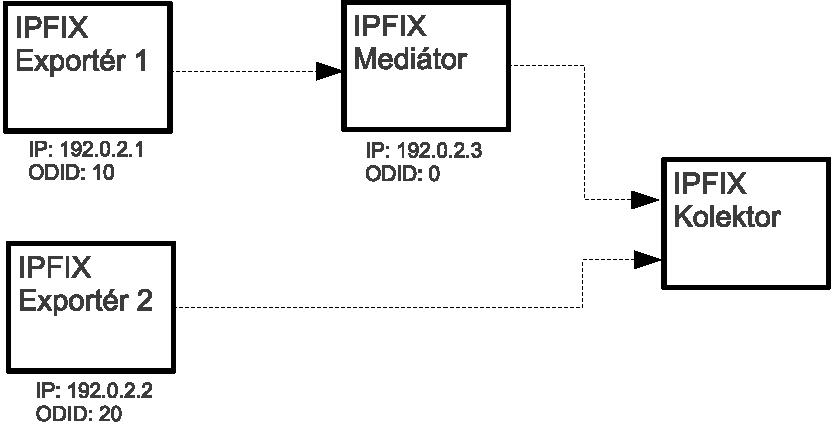
\includegraphics[width=0.7\textwidth]{loss_of_exporter}
\caption{Strata informácie o originálnom exportéri}\label{o:loss_of_exporter}
\end{figure}


\paragraph{Strata informácie o čase exportu} \label{sec:loss_time}

Pole čas exportu \emph{export time}, ktoré je zahrnuté v hlavičke správy predstavuje referenčnú 
časovú známku dátové záznamy. Niektoré informačné elementy popísané v \citep{rfc5102} nesú 
časové známky delta \emph{delta timestamps}, ktoré udávajú časový rozdiel voči hodnote v poli 
čas exportu. Ak dátový záznam zahŕňa nejaké pole s časovou známkou delta a Mediátor prepíše hodnotu 
času exportu,  tak časová známka delta týmto stráca význam. Kolektor však túto situáciu nevie 
rozpoznať a tak pracuje so zlými hodnotami.


\paragraph{Interpretácia sprostredkovaných správ}

V niektorých prípadoch potrebuje kolektor vedieť, ktoré konkrétne operácie resp. funkcie vykonal Mediátor 
nad dátovými záznamami. Kolektor nedokáže rozlíšiť medzi spájaním času a spájaním priestoru, v prípade, že 
Mediátor neexportuje použitú funkciu. Niektoré parametre vzťahujúce sa k funkcii by tiež mali byť 
exportované. 

V prípade spájania času, kolektor musí poznať aktívny timeout \emph{active timeout} 
pôvodných záznamov o tokoch. Pri spájaní priestoru je potrebné poznať nad akou oblasťou bola 
vykonaná kompozícia dátových záznamov.\citep{rfc5982}


%
\subsection{Analýza aplikačného rámca pre IPFIX Mediátor} \label{sec:framework}

Analýze aplikačného rámca pre sprostredkovanie správ v IPFIX sa venuje RFC 6183 \citep{rfc6183}. 
V jednotlivých kapitolách si podrobnejšie priblížime referenčný model, vybrané funkčné bloky 
aplikačného rámca a TODO ...

\subsubsection{Referenčný model sprostredkovania správ v IPFIX}

\begin{figure}[ht!]
\centering
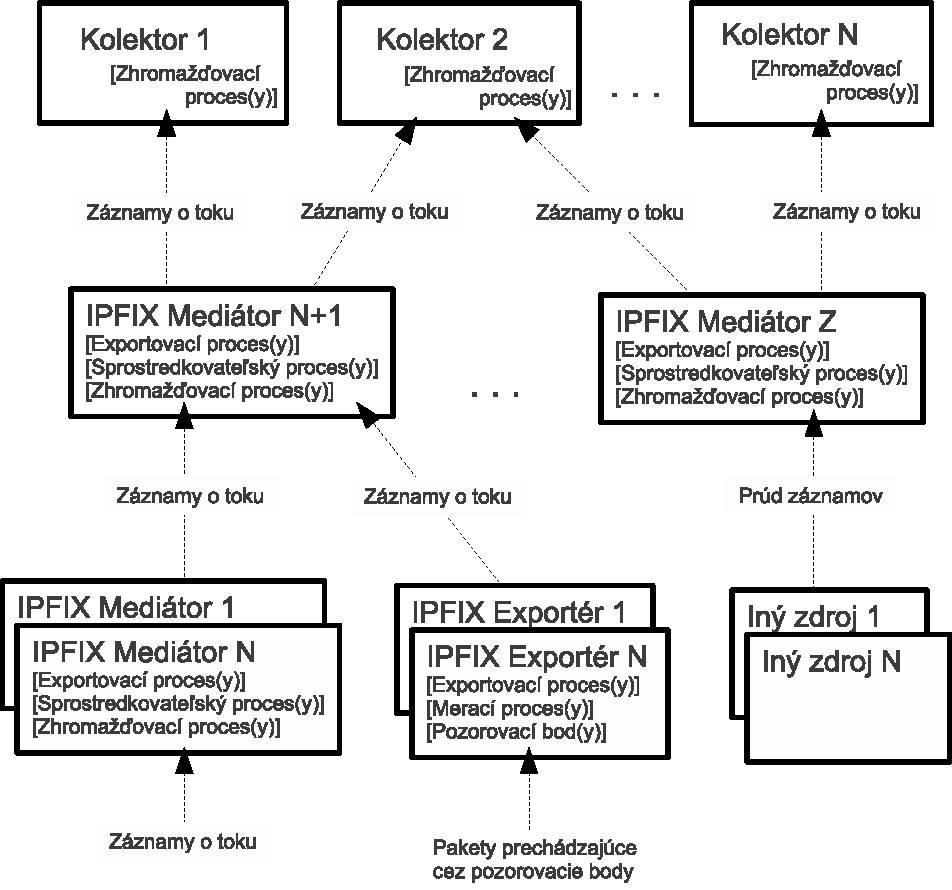
\includegraphics[width=0.9\textwidth]{mediation_reference_model}
\caption{Referenčný model sprostredkovania správ v IPFIX}\label{o:mediation_reference_model}
\end{figure}

Obrázok \ref{o:mediation_reference_model} predstavuje referenčný model sprostredkovania správ v IPFIX 
ako rozšírenie referenčného modelu IPFIX, popísaného v \emph{Architecture for IP Flow Information Export} 
\citep{rfc5470}. Táto schéma zobrazuje možné scenáre, ktoré môžu existovať v meracej architektúre.

Funkčné komponenty v rámci každej entity sú ohraničené zátvorkami []. Mediátor môže prijímať 
záznamy o toku od iných mediátorov a exportérov a prúd záznamov z iných zdrojov.
Za iné zdroje sa považujú nástroje iných protokolov, ako napríklad NetFlow exportéry \citep{rfc3954}. 
Spracovane dáta vo forme záznamov o toku potom exportuje jednému alebo viacerým kolektorom a mediátorom.

\begin{figure}[ht!]
\centering
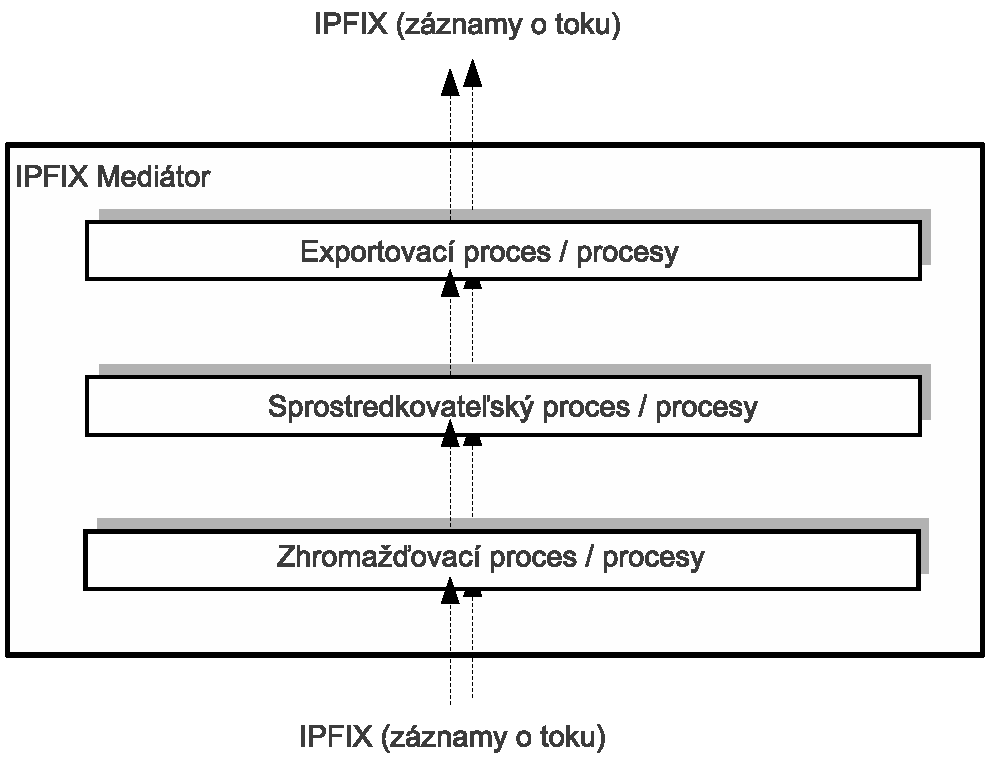
\includegraphics[width=0.7\textwidth]{mediator_component_model}
\caption{Zjednodušený model komponentov IPFIX Mediátora}\label{o:mediator_component_model}
\end{figure}

Zjednodušený model komponentov IPFIX mediátora je zobrazený na obrázku \ref{o:mediator_component_model}. 
Mediátor obsahuje jeden alebo viac sprostredkovateľských procesov, hierarchicky uložených 
medzi jedným alebo viacerými exportovacími a zhromažďovacími procesmi. Tento model sa týka 
najbežnejšieho prípadu, kedy mediátor prijíma dátové záznamy od exportéra, alebo iného mediátora.


\subsubsection{Komponenty sprostredkovania správ v IPFIX}

V nasledujúcich častiach si bližšie priblížime jednotlivé komponenty IPFIX mediátora, ktoré sú
znázornene na obrázku \ref{o:mediator_component_model}.

\paragraph{Zhromažďovací proces}

Zhromažďovací proces v IPFIX Mediátore sa nelíši od zhromažďovacieho procesu popísaného v 
špecifikácii IPFIX protokolu \citep{rfc5101}.
Jedinou funkciou naviac je odovzdanie sady dátových záznamov a riadiacich informácii jednému, alebo 
viacerým komponentom, tj. sprostredkovateľským procesom, alebo ďalším aplikáciam. 
To znamená, že zhromažďovací proces môže vytvárať kópie sady a prenášať ich buď sériovo, alebo paralelne.  
Medzi riadiace informácie patrí hlavička IPFIX správy, informácie o transportnej relácii, 
spolu s informáciami o meracom a exportovacom procese v exportéri, napr. vzorkovacie parametre.

\paragraph{Exportovací proces} \label{sec:exporting_process}

Exportovací proces IPFIX Mediátora sa vo svojej podstate tiež nelíši od toho, ktorý je popísaný v špecifikácii
protokolu \citep{rfc5101}.
Prídavné funkcie môžu byť nasledujúce:
\begin{itemize}
 \item Prijímať spúšťač \emph{trigger} od sprostredkovateľských procesov, ktorý vyvolá odoslanie správy
 kolektoru na odstránenie neplatnej šablóny \emph{(Template Withdrawal Message)}.
 \item Z dôvodu uvedeného v kapitole \ref{sec:loss_info} na strane \pageref{sec:loss_info}, je potrebné 
 preposielať informácie o pôvodcovi dat (exporterovi), napríklad ID pozorovacieho bodu a pozorovacej 
 domény, IP adresa exportéra atď. Tieto dáta zakóduje do prídavných dátových záznamov, bud s využitím 
 informačných elementov skupiny 2 (tabuľka \ref{t:ie-group2}), alebo organizáciou špecifikovaných 
 elementov.
\end{itemize}

% ---- tabuľka ----
\tabcolsep=8pt
\begin{table}[!ht]\caption{Prehľad informačných elementov skupiny 2}\label{t:ie-group2}
\smallskip
\centering
\begin{tabular}{|c|c|}
\hline
\textbf{ID} & \textbf{názov informačného elementu} \\ \hline
130 & exporterIPv4Address \\ \hline
131 & exporterIPv6Address \\ \hline
217 & exporterTransportPort \\ \hline
211 & collectorIPv4Address \\ \hline
212 & collectorIPv6Address \\ \hline
213 & exportInterface \\ \hline
214 & exportProtocolVersion \\ \hline
215 & exportTransportProtocol \\ \hline
216 & collectorTransportPort \\ \hline
173 & flowKeyIndicator \\ \hline
\end{tabular}
\end{table}
% -----------

\paragraph{Sprostredkovateľské procesy} \label{sec:framework_intermediate}

Sprostredkovateľské procesy sú kľúčovými funkčnými blokmi sprostredkovania správ v IPFIX. Musia pokryť 
každý príklad použitia sprostredkovania správ z kapitoly \ref{sec:mediator_examples} na strane 
\pageref{sec:mediator_examples}. 
Mediátor musí byť schopný súčasne podporovať viac ako jeden sprostredkovateľský proces. Spolupráca viacerých 
procesov je konfigurovaná nasledujúcimi spôsobmi.

\begin{itemize}
 \item \textbf{Paralelné spracovanie} - Prúd záznamov je spracovaný viacerými sprostredkovateľskými procesmi 
 paralelne tak, aby boli splnené požiadavky koncových aplikácií. V tomto scenári, každý 
 sprostredkovateľský proces dostáva kópiu celého prúdu záznamov ako vstup.
 \item \textbf{Sériové spracovanie} - Aby bolo zabezpečené flexibilné spracovanie prúdu záznamov, sprostredkovateľské
 procesy sú zapojene sériovo. V tomto prípade výstupný prúd záznamov jedného procesu je vstupným prúdom 
 nasledujúceho procesu.
\end{itemize}























%
\section{Projekty v\'yskumnej skupiny MONICA}

\subsection{Meracia plaforma BasicMeter}

BasicMeter \citep{monica} je jedným z projektov výskumnej 
skupiny MONICA, sídliacej v Laboratóriu počítačových sieti (CNL) na Technickej Univerzite v Kosiciach. 
Je to meraci nástroj zalozeny na protokole IPFIX. Sluzi na pasivne meranie parametrov prevadzky 
pocitacovych sieti a ich nasledne vyhodnocovanie. Zaciatky vyvoja siahaju az do roku 2003. Jeho 
architektura je znazornena na obrazku \ref{o:bm_architecture}.

\begin{figure}[ht!]
\centering
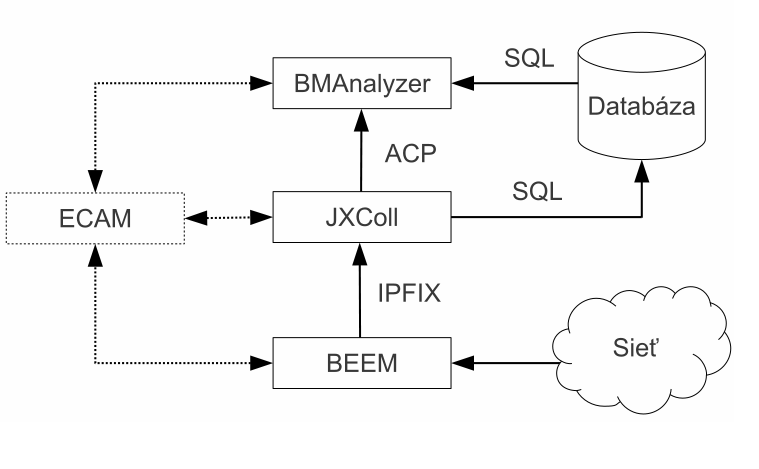
\includegraphics[width=0.7\textwidth]{bm_architecture}
\caption{Architektúra nástroja BasicMeter \citep{ja}}\label{o:bm_architecture}
\end{figure}

Platforma pozostava z nasledujucich komponentov:
\begin{itemize}
 \item \textbf{BEEM} - merací a exportovací proces - exporter
 \item \textbf{JXColl} - zhromažďovací proces - kolektor
 \item \textbf{BMAnalyzer} - aplikácia na vyhodnocovanie údajov
 \item \textbf{ECAM} - riadiaci komponent nástroja
 \item \textbf{bmIDS} - system pred detekciu narusenia
\end{itemize}

Najnizsou vrstvou architekury je \emph{BEEM}. Zabezpecuje vsetky funkcie 
meracieho a exportovacieho procesu definovaneho v specifikacii IPFIX. Namerané záznamy o tokoch
posiela komponentu \emph{JXColl} vo formate IPFIX sprav. Kolektor dekoduje prijate spravy od jedneho
alebo viacerych exporterov a uklada ich do databazy kvoli neskorsej analyze. Za ucelom analyzovania dat
a ich grafickeho zobrazenia vo forme grafov v realnom case ich posiela \emph{BMAnalyzeru} prostrednictvom 
protokolu ACP \citep{ado}. \emph{bmIDS} tak isto prijima data v realnom case, no jeho ulohou je analyzovat
prebiehajucu komunikaciu v uzli siete a odhalovat pripadne utoky, resp. anomalie. \emph{ECAM} umoznuje 
centralne riadit beh jednotlivych casti architektury. Umoznuje vytvorit a zmazat instancie exporterov 
a kolektorov, pripadne menit ich konfiguraciu. \citep{ja, veri}

\subsection{Merací nástroj SLAmeter}

SLAmeter je merač parametrov sieťovej prevádzky vyhodnocujúci dodržiavanie zmluvy o úrovni poskytovanej 
služby \emph{(SLA)}. V tomto prípade sa pod poskytovanou službou rozumie prístup do siete 
Internet. Zaklad nastroja zaklad je postaveny na komponentoch nastroja BasicMeter, a rovnako je projektom 
vyskumnej skupiny MONICA. 

Cieľom nástroja je spracovať vybrané parametre sieťovej prevádzky a vypočítať z nich akúsi triedu 
kvality. SLAmeter slúži každému, kto si chce skontrolovať kvalitu svojho pripojenia do Internetu. 
Triedy umožňujú jednoduchý spôsob porovnávania jednotlivých pripojení ponúkané poskytovateľmi, 
co by malo mat dopad na konkurenčný boj a zvýšenie snahy o zlepšovanie kvality služieb. \citep{slameter}

Ako bolo spomenute, SLAmeter je akousi nadstavbou na BasicMeter. Jeho architektura pozostava z exporterov,
ktore posielaju namerane zaznamy o tokoch zhromazdovacu. Ten spracovava zaznamy a uklada ich do 
centralnej databazy. Ulohou \emph{vyhodnocovaca} je na zaklade poziadaviek od weboveho rozhrania 
spracovavat IPFIX zaznamy a vytvarat tak statisticke a analyticke udaje o charaktere 
meranej sietovej prevadzky \citep{evaluator}. \emph{Webove rozhranie} je modularna webova aplikacia 
s pohladmi pre zakaznika a poskytovatela Internetovych sluzieb.
%
\section{Návrh a implementácia aplikačného rámca pre IPFIX Mediátor} \label{sec:navrh}

Na základe analýzy aplikačného rámca pre sprostredkovanie správ v~IPFIX, pozri Kapitolu~\ref{sec:analyza} 
(Sekcia~\ref{sec:framework}) a analýzy exportovacieho a zhromažďovacieho procesu v~RFC 5101
\citep{rfc5101} boli zhrnuté požiadavky a navrhnutá samotná architektúra IPFIX Mediátora. 
Jeho jednotlivým komponentom, ktoré sú vyššie znázornené na~Obrázku~\ref{o:mediator_component_model} 
a požiadavkám sú venované nasledujúce kapitoly. Upozorňujeme, že termíny \uv{sprostredkovateľský proces}, 
\uv{sprostredkovateľský modul}, resp. \uv{modul} sú úplne totožné a zameniteľné.


\subsection{Požiadavky na rámec pre IPFIX Mediátor}

\begin{itemize}
 \item \textbf{Modulárna implementácia} -- už počas analýzy sprostredkovania správ v IPFIX bolo zrejmé, že 
 aplikačný rámec musí byť modulárny. Musí mať podporu pre jednoduché a flexibilné pridávanie resp. 
 odoberanie modulov. Opäť zdôrazňujeme, že predstaviteľom modulu je sprostredkovateľský proces.
 
  \item \textbf{Oddelenie logiky rámca od logiky sprostredkovateľských procesov} -- 
  najdôležitejšie je, aby budúci riešitelia sprostredkovateľských procesov nemuseli vôbec zasahovať 
  do zdrojového kódu aplikačného rámca. Všetky potrebné metódy pre prácu so záznamami o~tokoch 
  im musí zabezpečiť rámec, ale rovnako im musí zakázať prístup k~jeho interným metódam. 
  Iba tak môže byť zachovaná jednotnosť prístupu. Nie je možné, aby každý sprostredkovateľský proces 
  riešil napr. zakódovanie, alebo dekódovanie dátových záznamov po svojom. Preto je potrebné navrhnúť 
  a implementovať rozhranie, prostredníctvom ktorého budú procesy komunikovať s~aplikačným rámcom.
  
 \item \textbf{Dynamické načítavanie sprostredkovateľských procesov} -- pridávanie a odoberanie 
 sprostredkovateľských procesov musí byť riadené výlučne cez konfiguračný súbor. Nesmie byť potrebný 
 žiadny zásah do zdrojového kódu  rámca.
 
 \item \textbf{Jednoduchá konfigurácia} -- ako už bolo spomenuté v~analýze -- Kapitola~\ref{sec:analyza} 
 (Sekcia~\ref{sec:framework_intermediate}), 
 sprostredkovateľské procesy spracúvajú prijaté záznamy o~tokoch bud sériovo, alebo paralelne. 
 Celková štruktúra odovzdávania dát v~rámci mediátora od zhromažďovacieho procesu, sériovo a paralelne cez 
 všetky procesy a napokon až k~exportovaciemu procesu musí byť jednoznačne konfigurovateľná v~textovom 
 XML súbore a v~čo najviac používateľsky priateľskom formáte. 
 
 \item \textbf{Distribúcia dát medzi komponentmi} -- aplikačný rámec musí zabezpečiť spôsoby prenosu dát medzi 
 jednotlivými sprostredkovateľskými procesmi, zhromažďovacím a exportovacím procesom. Tieto spôsoby 
 musia byť pre procesy jednotné a bez možnosti zmeny z~vnútra sprostredkovateľského procesu.
 
 \item \textbf{Jediná inštancia modulov} -- bolo navrhnuté, že každý sprostredkovateľský
 proces musí byť implementovaný podľa návrhového vzoru \emph{Singleton}. Je to z~toho dôvodu, že 
 každý proces musí byť unikátny a jednoznačne rozpoznateľný v~rámci celého programu na 
 základe mena triedy procesu. Konfigurácia toku dát cez procesy spomínaná vyššie bude daná práve 
 prostredníctvom názvov ich tried. Jedinečnosť procesov musí zabezpečiť aplikačný rámec. 
 
 \item \textbf{Jednotné dekódovanie a zakódovanie dátových záznamov} -- aplikačný rámec musí obsahovať metódy 
 prístupné všetkým sprostredkovateľským procesom, ktoré budú dekódovať dátové záznamy na dáta a opačne
 na základe šablón.
 
 \item \textbf{Viacvláknovosť} -- nielen zo samotnej povahy paralelných procesov, ale aj modularity vyplýva, 
 že každý sprostredkovateľský proces bude vykonávaný v~samostatnom vlákne, prípadne viacerých vláknach. 
 Podobne zhromažďovací a exportovací proces budú rozdelené na viac vlákien. 
 
 \item \textbf{Konformita s~protokolom IPFIX} -- výstupom Mediátora musia byť správy zakódované 
 v~konformite so špecifikáciou IPFIX protokolu. Kolektor spracováva správy prijaté od Mediátora rovnakým
 spôsobom, akoby ich prijal od~exportéra. Navyše zhromažďovací a exportovací proces aplikačného rámca sa 
 nesmú líšiť od charakteristík týchto procesov daných špecifikáciou IPFIX protokolu v~RFC 
 5101 \citep{rfc5101}.
 
 \item \textbf{Komunikácia pomocou UDP} -- v~tejto fáze projektu bol zvolený ako komunikačný protokol UDP.
 Dôvodom bola rýchlosť, jednoduchosť a dobré skúsenosti s~implementáciou UDP v~JXColl. Napriek tomu, že 
 UDP nie je  spojovo orientovaný transportný protokol, v~prípade nasadenia Mediátora v~SLAmetri to vôbec
 nevadí. Mediátor bude nasadený fyzicky na tej istej lokálnej sieti ako exportér a kolektor. 
 
 \item \textbf{Programovací jazyk Java} -- pre implementáciu bol vybratý programovací jazyk Java.
 Hlavným dôvodom bol fakt, že zhromažďovací proces Mediátora a IPFIX kolektora sú veľmi podobné a JXColl 
 je naprogramovaný v~tomto jazyku. Ďalším faktom je relatívne jednoduchá tvorba modulárnych aplikácii,
 vďaka načítavaniu tried pomocou \emph{Java ClassLoader}. V~neposlednom rade zohrala svoju rolu aj vysoká
 podpora jazyka Java, či už sa jedná o~kvalitu dokumentácie, veľké množstvo odborných fór, dostupnosť 
 knižníc jazyka, ale aj fakt, že Java aplikácie sú spustiteľné na väčšine operačných systémov.
\end{itemize}

%% -------------------- MEDIATOR -----------------

\subsection{Hlavn\'a trieda Medi\'atora}


Úlohou hlavnej triedy Mediátora je postupne spustiť všetky svoje vlákna a procesy potrebné pre beh 
programu. Najprv sa prečítajú a spracujú argumenty príkazového riadku. Program vie rozpoznávať dva druhy 
argumentov. Jedným z~nich je cesta ku konfiguračnému súboru. Ak nie je zadaná, používa sa východiskový 
konfiguračný súbor. Druhým argumentom môže byť zadaná možnosť \verb|--logtofile|. Vtedy sú všetky 
logovacie výstupy presmerované zo štandardného výstupu do súboru.

Potom ako program načíta všetky nastavenia z~konfiguračného súboru, spustí svoje moduly -- 
sprostredkovateľské procesy pomocou triedy \verb|IPLoader|. Nasleduje spustenie vlákna, ktoré prijíma 
IPFIX pakety prostredníctvom protokolu UDP a vlákna, ktoré ich spracováva. Hovoríme o~\verb|UDPServer| 
a \verb|UDPProcessor|. Nakoniec je spustené exportovacie vlákno -- \verb|UDPExporter|. Kedykoľvek keď 
nastane chyba je Mediátor korektne ukončený a to tak, že uvoľní všetku pamäť a zastaví bežiace vlákna. 
Rovnako je Mediátor zastavený po stlačení kombinácie kláves \verb|Ctrl-c|.
Podrobne o~každom spomenutom vlákne a procese bude povedané v~nasledujúcich kapitolách.






%% -------------------- COLLECTING -----------------

\subsection{Zhromažďovací proces} \label{sec:collectingprocess}

Na základe analýzy a zhodnotenia požiadaviek na zhromažďovací proces bola navrhnutá jeho architektúra.
Logická štruktúra procesu sa skladá z~dvoch fáz, pričom každú fázu predstavuje jedno vlákno. 
Venujme sa teda jednotlivým fázam procesu.

\subsubsection{1. fáza zhromažďovacieho procesu}

Prvá fáza je znázornená na Obr. \ref{o:collecting1_schema} a predstavuje najnižšiu vrstvu celého 
nástroja. Jej jadrom je UDP server, bežiaci v~samostatnom vlákne. V~jeho hlavnej metóde \emph{run()}
cyklicky vykonáva kód, dokiaľ nie je prerušený výnimkou \emph{InterruptedException}.
Tento kód odchytáva údaje posielané protokolom UDP na úrovni bajtov a ukladá ich do 
vyrovnávacej pamäte. K~tomuto je použitý objekt triedy jazyka Java -- \verb|ByteBuffer|. Zároveň sa do 
objektu triedy \verb|InetSocketAddress| uloží IP adresa exportéra a zaznamená sa čas prijatia dát
v~milisekundách vo formáte časovej známky Unix-u \emph{(Unix Timestamp)}. Tieto tri premenné sú argumentom 
funkcie \emph{write()}, 
ktorá z~prijatých premenných vytvorí objekt typu \verb|PacketObject|. Tento objekt je akousi
abstraktnou reprezentáciou paketu, vo svojich členských premenných uchováva údaje z~hlavičky
IPFIX správy (sekvenčné číslo, čas exportu, ID pozorovacej domény) spolu s~obsahom správy, časom 
prijatia a adresy z~ktorej bol prijatý. Prijatá IPFIX správa sa v~tejto forme uloží do vyrovnávacej 
pamäte, ktorú predstavuje trieda \verb|PacketCache|. Jej členská 
premenná \emph{cache} je typu \verb|ArrayBlockingQueue|, čo je vlastne Java implementácia \emph{FIFO}
frontu, ktorý je navyše synchronizovaný a~optimalizovaný na vysoký výkon. Táto vyrovnávacia pamäť 
medzi prvou a druhou fázou zhromažďovacieho procesu je kritická vo vysoko rýchlostných sieťach. 

\begin{figure}[ht!]
\centering
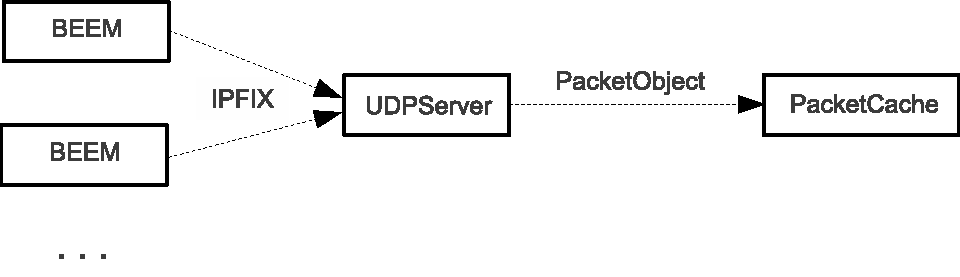
\includegraphics[width=0.8\textwidth]{collecting1_schema}
\caption{Schéma prvej fázy zhromažďovacieho procesu Mediátora}\label{o:collecting1_schema}
\end{figure}

Návrh umožňuje do budúcna jednoduchú rozšíriteľnosť programu o~triedy implementujúce servery iných transportných 
protokolov, napr. TCP a SCTP. Tieto servery budú rovnako ako \verb|UDPServer| bežiace v~samostatných 
vláknach.

\subsubsection{2. fáza zhromažďovacieho procesu}

Schému druhej fázy vidíme na Obr. \ref{o:collecting2_schema}. Hlavná metóda \emph{run()} vlákna 
\verb|UDPProcessor| cyklicky vyberá dáta z~\verb|PacketCache| a odovzdáva ich \emph{parseru}. 
Ten je reprezentovaný 
triedou \verb|IPFIXParser|. Správy číta z~vyrovnávacej pamäte dokiaľ nie je prerušený výnimkou 
\emph{InterruptedException}.
UDP procesor robí zároveň kontrolu, či prijaté dáta sú IPFIX paketom. V~tomto prípade, ale aj v~prípadoch
keď prijaté dáta sú poškodené sa správa zahadzuje a program pokračuje spracovávaním ďalšej správy.
Trieda \verb|IPFIXParser| sa používa na spracovanie prijatých paketových binárnych dát, ktorého 
výsledkom je hotový objekt IPFIX správy, obsahujúci všetky jej komponenty, pozri 
Kapitolu~\ref{sec:analyza} (Sekcia~\ref{sec:message_format}). Metódy tejto triedy najprv vyskladajú 
kompletnú hlavičku správy a potom sa pustia do parsovania IPFIX sád. Na základe identifikátora sady 
spracujú a vytvoria objekty pre sadu šablón, sadu šablón možností a dátovú sadu. Sady následne naplnia 
príslušnými záznamami. 

\begin{figure}[ht!]
\centering
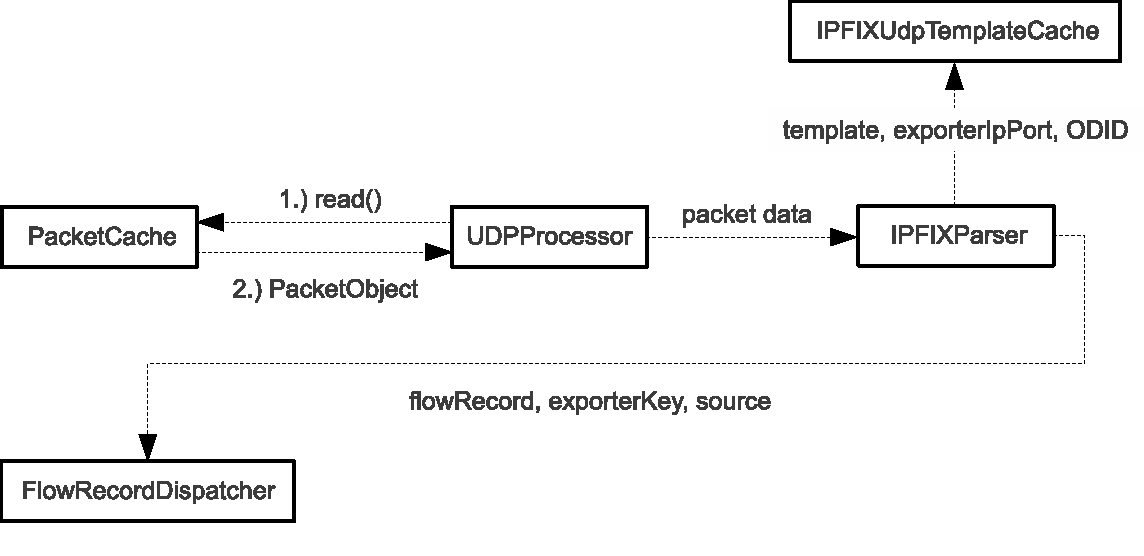
\includegraphics[width=0.8\textwidth]{collecting2_schema}
\caption{Schéma druhej fázy zhromažďovacieho procesu Mediátora}\label{o:collecting2_schema}
\end{figure}

Prichádzajúce záznamy šablón a záznamy šablón možnosti sú posielané špecializovanej triede 
\verb|IPFIXUdpTemplateCache|, ktorá má na starosti správu prijatých šablón osobitne pre každý exportér. 
Ako je zrejmé zo špecifikácie exportovacieho procesu, šablóna musí byť odoslaná kolektoru okamžite ako je 
vytvorená a ešte pred odoslaním jej prislúchajúcich dátových záznamov. Potom je šablóna periodicky 
preposielaná. Trieda \verb|IPFIXUdpTemplateCache| nové šablóny ukladá. Objekty šablón, ktoré už má 
uložené ale aktualizuje. Zároveň maže staré šablóny, ku ktorým nedostala aktualizáciu po dobu definovanú
v~konfiguračnom súbore.

Napokon sa každý dátový záznam v~dátovej sade, s~prislúchajúcou šablónou a hlavičkou IPFIX správy 
zabalí do objektu triedy \verb|IPFIXFlowRecord|, ktorá je reprezentáciou záznamu o~toku. 
Tento záznam spolu s~reťazcom, ktorý určuje odkiaľ záznam vystupuje \emph{(inputProcess)} sú posielané
ako parametre triede \verb|FlowRecordDispatcher|. V~tomto prípade reťazec, ktorý určuje pôvodcu záznamu 
je \emph{\uv{exporter}}. 
Dispečer záznamov o~tokoch -- \verb|FlowRecordDispatcher| rozdistribuuje prijaté záznamy o~tokoch 
príslušným sprostredkovateľským procesom, alebo ich pošle na export. O~tom podrobnejšie v~samostatnej 
Kapitole~\ref{sec:navrh} (Sekcia~\ref{sec:FlowRecordDispatcher}). 

%% -------------------- COLLECTING END -----------------
%% -------------------- INTERMEDIATE -----------------

\subsection{Rozhranie a podpora pre sprostredkovateľské procesy -- moduly} \label{sec:intermediate_process}

Vyššie boli definované viaceré požiadavky na sprostredkovateľské procesy, ktoré musí zabezpečiť 
aplikačný rámec. Hovoríme o~modulárnej implementácii, oddelení logiky rámca od logiky procesov, 
ich dynamickom načítavaní, jedinej inštancii procesov atď. Riešenie týchto požiadaviek bude vysvetlené
v~nasledujúcich kapitolách. Začnime ale najprv teoretickým základom dynamického načítavania tried.

\subsubsection{Java ClassLoader a dynamické načítavanie tried} \label{sec:classLoader}

\emph{Java ClassLoader} je súčasťou \emph{Java Runtime Environment} (JRE) a jeho úlohou je dynamické
načítavanie tried jazyka Java do \emph{Java Virtual Machine} (JVM) na základe ich mena. 
Načítavanie tried je jeden zo základných a najsilnejších mechanizmov, ktorý poskytuje programovací jazyk
Java. Vďaka nemu JRE nemusí vedieť nič o~súboroch a súborovom systéme počas vykonávania Java programov. 
Navyše tieto súbory tried nie sú načítavané do pamäte naraz, ale podľa požiadaviek 
programu. \citep{mcmanis, travis}

Načítavanie tried je organizované do stromovej štruktúry. Koreňom štruktúry je samozavádzací 
\emph{(bootstrap) class loader}, ktorý je napísaný v~natívnom kóde a nie je možné vytvárať jeho inštancie. 
Vytvára ho 
JVM a je zodpovedný za načítanie interných tried Java Development Kit (JDK) a \emph{java.*} balíčkov 
obsiahnutých v~JVM. Príkladom je \verb|java.lang.String|. Potomkom samozavádzacieho loadera je 
\emph{extension class loader},
ktorého primárnou zodpovednosťou je načítavať triedy z~\emph{extension} priečinkov. Toto je pohodlný 
spôsob rozšírenia JDK bez pridávania položiek do premenných prostredia -- \emph{CLASSPATH}. 
Rozšírením \emph{extension classloader-a} je aplikačný, resp. \emph{systémový class loader}. Jeho úlohou 
je načítanie tried z~cesty danej premennou prostredia. Inštanciu systémového class loadera získavame 
metódou \verb|ClassLoader.getSystemClassLoader()|. \citep{techjava, antl}

Abstraktná trieda \verb|ClassLoader| je umiestnená v~balíčku \verb|java.lang|. Vývojári môžu pridať 
vlastnú 
funkcionalitu do načítavania tried vytvorením vlastnej, ktorá bude rozšírením triedy 
\verb|ClassLoader|. Typickou stratégiou je transformovanie mena triedy na meno súboru a následné 
prečítanie \uv{súboru triedy} \emph{(class file)} zo súborového systému. \citep{christudas, classloader}

Na dynamické načítavanie tried na základe ich binárneho mena sa používa metóda \verb|loadClass(String name)|.
Táto metóda bola použitá pri načítavaní modulov definovaných v~konfiguračnom súbore a aj pri získavaní 
inštancií sprostredkovateľských procesov, ktoré boli potrebné pri riadení toku dát medzi procesmi.
Podrobnejšie sa tomu venujeme v~príslušných kapitolách. 



\subsubsection{Abstraktná trieda AIntermediateProcess} 

Po analýze požiadaviek bolo jasné, že je potrebné pripraviť akési rozhranie pre~sprostredkovateľské 
procesy, ktoré by oddeľovalo ich logiku od logiky aplikačného rámca. Navyše toto rozhranie musí 
definovať základné vlastnosti, ktoré sú rovnaké pre všetky procesy a implementovať metódy, ktoré 
majú byť procesom dostupné. Jednoznačnou odpoveďou na tieto otázky je abstraktná trieda, 
od ktorej budú všetky moduly dediť. 


\paragraph{Viacvláknovosť}
Každý modul musí byť vykonávaný v~samostatnom vlákne. Preto trieda \verb|AIntermediateProcess| dedí
od triedy \verb|Thread| a obsahuje abstraktnú metódu \emph{run()}, čo je vlastne deklaráciou 
hlavnej metódy vlákien. Toto zabezpečí, že v~každom module bude musieť byť jej konkrétna implementácia.


\paragraph{Jediná inštancia modulov} \label{sec:singleton}
Ďalšou požiadavkou bolo, že moduly musia byť implementované podľa návrhového vzoru Singleton. V~prípade, že
by existovalo viacero inštancií každého modulu, trieda \verb|FlowRecordDispatcher| by nemohla správne 
distribuovať záznamy o~tokoch medzi procesmi. Vzorová implementácia návrhového
vzoru singleton je nasledovná:  
\begin{verbatim}
 public class Singleton {
    private static Singleton instance = null;
 
    private Singleton() {}
 
    public static Singleton getInstance() {
            if (instance == null) {
                   instance = new Singleton();
            }
            return instance;
   }
}
\end{verbatim}
Nedá sa spoľahnúť na to, že budúci vývojári modulov budú implementovať sprostredkovateľské procesy 
podľa tohoto návrhového vzoru, preto to musí zabezpečiť aplikačný rámec, presnejšie trieda od ktorej 
dedia -- \verb|AIntermediateProcess|.
Bohužiaľ, v~jazyku Java nie je možné, aby Singleton implementovala abstraktná trieda, hneď z~viacerých
dôvodov (vymenované len niektoré):
\begin{enumerate}
 \item Singleton vyžaduje konštruktor s~viditeľnosťou \emph{private}. Toto sa vylučuje s~možnosťou 
 dedenia od abstraktnej triedy.
 \item Členská premenná \verb|instance| je typu \emph{static}. Teda sa viaže k~triede Singleton a nie k~jej 
 potomkom.
 \item V~prípade, že členská premenná \verb|instance| má hodnotu \emph{null}, je potrebné vytvoriť novú inštanciu 
 potomka a nie rodičovskej triedy. Avšak inštanciu ktorého potomka?
 \item Druhý prístup je deklarovať metódu \emph{getInstance()} abstraktnou. Konkrétna implementácia 
 by tak bola zabezpečená triedami sprostredkovateľských procesov, premenná \verb|instance|
 by bola správneho typu. Tento návrh je však nerealizovateľný. 
 Metóda \emph{getInstance()} rodičovskej triedy nemôže byť statická a zároveň abstraktná. V~jazyku Java
 to nie je možné. 
 \emph{Static} metóda patrí triede, kde je definovaná. 
 Pričom \emph{abstract} naznačuje, že funkcionalita bude definovaná až v~potomkoch. Tu dochádza
k~logickému rozporu.
\end{enumerate}
Preto bolo potrebné navrhnúť a implementovať iný spôsob, ktorý by zabezpečil jedinú inštanciu pre všetky 
moduly z~abstraktnej rodičovskej triedy. Riešenie navrhol britský Java programátor \emph{Niall Gallagher}
na jednom z~diskusných fór o~probléme dedenia a návrhového vzoru Singleton \citep{gallagher}.
Jeho riešenie je hybridom viacerých prístupov, ktoré sa diskutujú na Internete, no vychádza
z~návrhového vzoru \emph{Factory method}. Výsledkom je abstraktná trieda, slúžiaca ako továreň na 
podtriedy tým, že volá jej statická metóda \emph{getInstance(Class clazz)}. 
\begin{verbatim}
private static final Map singletonRegistry = new HashMap();

public static final synchronized 
<T extends AIntermediateProcess> T getInstance(Class clazz) {
  T instance = (T) singletonRegistry.get(clazz);
  if (instance == null) {
      try {
          instance = (T) clazz.newInstance();
      } catch (InstantiationException | IllegalAccessException ex) {
          log.error(ex);
      }
      if (instance != null) {
          singletonRegistry.put(clazz, instance);
      } else {
         log.error(Could not register singleton);
      }
 }
 return instance;
}
\end{verbatim}
Ak sú splnené podmienky, že konkrétna trieda, napr. \verb|SelectionProcess| je definovaná v~rovnakom 
balíčku ako \verb|AIntermediateProcess| a ich konštruktory nemajú explicitne nastavený prístup 
(predvoleným prístupom je \uv{privátny v~rámci balíčka}), tak 
jediným spôsobom ako získať inštanciu podtriedy mimo balíčka je cez konštrukciu:
\begin{verbatim}
 SelectionProcess instance = 
 AIntermediateProcess.getInstance(SelectionProcess.class);
\end{verbatim}
Dalo by sa vyčítať, že vytváranie inštancií používa reflexiu, ktorá je pomalá. Avšak, keďže vytvárame 
Singleton-y, volanie \emph{newInstance()} sa vykoná pre každý modul práve raz.

Aby bolo možné získavať inštancie modulov aj na základe mena triedy a nie len cez \emph{class} objekty, bola 
vytvorená ďalšia metóda \emph{getInstance(String processName)}. Parameter \emph{processName} je práve meno 
procesu, napr \verb|SelectionProcess|. Táto premenná sa prevedie na binárne meno procesu, 
podľa špecifikácie jazyka Java \citep{java_spec},
napr. \verb|sk.tuke.cnl.Mediator.SelectionProcess|.
Prostredníctvom systémového class loadera, tak ako to bolo vyššie spomínané, sa z~binárneho mena 
sprostredkovateľského procesu získa jeho \emph{class} objekt. Potom sa zavolá pôvodná metóda 
\emph{getInstance(Class clazz)} a tá vráti inštanciu procesu.
\begin{verbatim}
 String name = Default.PROCESSES_LOCATION + processName;
 Class clazz = ClassLoader.getSystemClassLoader().loadClass(name);
 instance = AIntermediateProcess.getInstance(clazz);
\end{verbatim}



\paragraph{Dekódovanie dátových záznamov} 
Bola vyslovená požiadavka, že aplikačný rámec musí obsahovať metódy pre dekódovanie a zakódovanie 
dátových záznamov na základe šablón. Nie je žiadúce, aby v~budúcnosti každý vývojár sprostredkovateľských 
procesov riešil tieto úlohy po svojom. 

Už v~konštruktori triedy sa získa inštancia triedy \verb|IPFIXElements|, ktorá poskytuje 
funkcie na jednoduché získanie informácii o~podporovaných informačných elementoch. Trieda sparsuje XML 
súbor \emph{(ipfixFields.xml)} a dáta uloží do hash mapy, ktorá používa mapovanie z~ID informačného 
elementu na objekt typu \verb|IpfixField|. Tento objekt obsahuje informácie o~elementoch, ako 
napríklad meno, dátový typ, meno skupiny do ktorej patrí a identifikačné číslo.\citep{veri}

Na dekódovanie slúži metóda \emph{decodeDataRecord()}, jej parametrami sú dátový záznam a príslušná
šablóna. V~prvej fáze je potrebné získať zakódovanú hodnotu z~dátového záznamu, druha fáza dekóduje 
bajty informačného elementu na hodnotu definovanú dátovým typom.

V~cykle sa prechádzajú všetky špecifikátory poľa v~šablóne. Na začiatku procesu sa pre každý 
špecifikátor určí číslo organizácie (ak je definované) a ID informačného elementu. Ak sa daný informačný
element nenachádza v~hash mape informačných elementov, tak je zaznamenaná chyba a pokračuje sa 
na spracovanie ďalšieho špecifikátora poľa. Potom sa získa meno, dátový typ a skupina informačného elementu. 
Posledne menované je skôr z~informačných dôvodov, kvôli logovacím výpisom. Následne sa určí pozícia 
špecifikátora poľa v~šablóne, pretože na rovnakej pozícii je uložená zakódovaná hodnota informačného
elementu v~dátovom zázname. Metóda teda získa tieto bajty, obalí ich do objektu triedy \emph{ByteBuffer}  
a ten pošle spolu s~pomenovaním dátového typu na dekódovanie triede \verb|IPFIXDecoder|.

Na základe dátového typu je určená metóda, ktorá dekóduje bajty obsiahnuté vo~vyrovnávacej pamäti.
Dekódovanie je implementované v~súlade s~RFC 5101 \citep{rfc5101} a 
RFC 5102 \citep{rfc5102} pre všetky dátové typy podporované protokolom IPFIX. Vymenujme aspoň niektoré:
znamienkové a bezznamienkové celé čísla na 8, 16, 32, 64 a 128 bitoch, čísla v~pohyblivej rádovej čiarke na 
32 a 64 bitoch, dátumy, IPv4 a IPv6 adresy, MAC adresy a pod. 

Dekódovaná hodnota je z~dekódera vrátená ako reťazec. Všetky hodnoty sa ukladajú do hash mapy, ktorá 
kvôli jednoduchému vyhľadávaniu prvkov asociuje názov informačného elementu na jeho hodnotu. 
Takáto dátová mapa so všetkými dekódovanými hodnotami z~dátového záznamu je vrátená sprostredkovateľskému 
procesu, ktorý si ju vyžiadal.


\paragraph{Zakódovanie dátových záznamov} 
Presným opakom predchádzajúcej metódy je metóda \emph{encodeDataRecord()}. Jej parametrami sú dátová 
mapa (výsledok dekódovania), príslušná šablóna a počet polí v~dátovom zázname, ktoré je potrebné 
zakódovať -- \emph{recordsCount}.

Na začiatku vykonávania metódy sa inicializuje pole objektov \emph{ByteBuffer} o~veľkosti \emph{recordsCount}.
Toto pole slúži ako pomocná premenná pre uchovávanie zakódovaných hodnôt. Zároveň sa vytvorí objekt 
nového dátového záznamu.
Následne sa v~cykle prechádzajú všetky hodnoty v~dátovej mape. Pri každom prvku sa získa jeho identifikátor
z~inštancie triedy \verb|IPFIXElements| na základe mena prvku. Vďaka tomu sa potom dá určiť číslo
organizácie, dátový typ a pozícia špecifikátora poľa v~šablóne. 

Keď sú určené všetky potrebné hodnoty, tak dátový typ a hodnota informačného elementu sú poslané triede 
\verb|IPFIXEncoder| na zakódovanie. Táto trieda bola navrhnutá a implementovaná analogicky k~dekóderu. 
Aj tu sú pokryté všetky dátové typy, ktoré podporuje IPFIX protokol vrátane jedného naviac -- bezznamienkového
celého čísla na 128 bitoch -- \emph{unsigned128}. Tento dátový typ využívajú niektoré informačné elementy 
definované Laboratóriom počítačových sietí na Technickej univerzite v~Košiciach. Podľa špecifikácie
\citep{rfc5101} musia byť zakódované informačné elementy posielané v~sieťovom poradí bajtov, známom 
tiež ako \emph{Big-Endian}. 

Na základe dátového typu je určená funkcia, ktorá vykoná kódovanie. 
Tieto funkcie musia uskutočniť radu kontrol, či je vstupná hodnota v~reťazci validná. 
Pri číselných typoch a dátumoch sa kontroluje správny rozsah a formát čísla, pri MAC adresách zase 
správny formát a podobne.
V~prípade, že vstupná kontrola nie je validná, je vyhodená príslušná výnimka a 
kódovanie je úplne ukončené, dátový záznam sa neexportuje. Je neprípustné, aby Mediátor posielal kolektoru
dátové záznamy s~prázdnymi hodnotami z~dôvodu, že nebolo možné zakódovať hodnotu danú v~zlom formáte.  

Pri kódovaní je veľmi dôležitá rýchlosť a pamäťová 
nenáročnosť kódovacích funkcií. Jedna funkcia, napr. na zakódovanie znamienkového celého čísla na 32
bitoch môže byť zavolaná veľakrát v~rámci kódovania jediného dátového záznamu. Tento počet zavisí od 
dátových typov informačných elementov v~dátovom zázname. Nemusíme zdôrazňovať aké množstvo IPFIX paketov 
a dátových záznamov môže Mediátor v~čase prijímať. Preto bol kladený veľký dôraz na to, aby boli 
kódovacie funkcie čo najoptimálnejšie. 

Ukážme si to na príklade. Úlohou je zakódovať znamienkové celé číslo $-42$ na pole štyroch bajtov.
Najjednoduchším a najpohodlnejším riešením je použiť triedu \emph{ByteBuffer}, alokovať pole veľkosti 
$4$ bajty, nastaviť poradie bajtov na \emph{Big-Endian}, vložiť číslo $-42$ a konvertovať na pole 
volaním \verb|array()|. Druhou možnosťou je použiť triedu \verb|BigInteger|, vložiť hodnotu $-42$, 
a konvertovať na pole bajtov. V~tejto metóde sa nedá explicitne nastavovať poradie bajtov, pole 
je stále zoradené v~\emph{Big-Endian}, čo nám vyhovuje. Nepríjemnosťou je dodatočné orezanie na 
potrebný počet bajtov. 
\begin{verbatim}
 ByteBuffer buf = ByteBuffer.allocate(4).order(ByteOrder.BIG_ENDIAN);
 byte[] b1 = buf.putInt(-42).array();
 
 byte[] b2 = BigInteger.valueOf(-42).toByteArray();
\end{verbatim}
Obe tieto metódy zbytočne pridávajú réžiu, zložitosť a zvyšujú pamäťovú náročnosť výpočtu tým, že 
používajú komplexné Java triedy. Preto boli pre všetky konverzie implementované metódy pomocou bitových
posunov a bitových operátorov. Tieto metódy prevádzajú všetky číselné primitívne typy jazyka Java 
(byte, short, int, long, float a double) na pole bajtov na najnižšej možnej úrovni, čo zabezpečuje vysoký
výpočtový výkon. Ukážme si túto konverziu na 4-bajtovom čísle $-42$.
\begin{verbatim}
 public static byte[] intToByteArray(int x) {
        return new byte[]{
            (byte) ((x >> 24) & 0xFF),
            (byte) ((x >> 16) & 0xFF),
            (byte) ((x >> 8) & 0xFF),
            (byte) (x & 0xFF)
        };
 }
 
 byte[] b3 = intToByteArray(-42);
\end{verbatim}

Hodnota zakódovaná na pole bajtov sa uloží do pomocného poľa spomínaného vyššie, na rovnakú pozíciu
ako je pozícia špecifikátor poľa v~šablóne. Keď sa prejdú všetky hodnoty pripravené na zakódovanie, 
pomocné pole je vyskladané v~správnom poradí a teda ho môžeme uložiť do objektu dátového záznamu.
Hotový dátový záznam je vrátený sprostredkovateľského procesu, ktorý si ho vyžiadal.


\paragraph{Distribúcia dát medzi modulmi} 
Trieda \verb|AIntermediateProcess| poskytuje rozhranie pre distribúciu záznamov o~tokoch medzi 
jednotlivými sprostredkovateľskými procesmi vďaka metóde \emph{dispatchFlowRecord()}. 
Jej jedinou úlohou je zavolanie rovnomennej metódy distribútora záznamov - triedy \verb|FlowRecordDispatcher|.
O~tom podrobne v~samostatnej Kapitole~\ref{sec:navrh} (Sekcia~\ref{sec:FlowRecordDispatcher}).



\subsubsection{Príklad implementácie modulu -- ExampleProcess}

Pre budúcich riešiteľov bol propravený jednoduchý príklad implementácie sprostredkovateľského procesu.
Predstavuje ho trieda \verb|ExampleProcess|, ktorej úlohou je veľmi jednoduchá anonymizácia zdrojovej a 
cieľovej IP adresy zmenením čísla posledného oktetu na nulu. 

Trieda demonštruje všetky pravidlá programovania sprostredkovateľských procesov. V~prvom rade dedí od 
abstraktnej triedy \verb|AIntermediateProcess|. Taktiež má konštruktor bez explicitne definovaného 
prístupu, v~ktorom volá rodičovský konštruktor so svojím menom ako parametrom. Toto síce nie je povinné,
ale zaistí to, že vlákno bude pomenované, teda v~príslušných logovacích výpisoch bude jeho meno.
V~opačnom prípade dostane vlákno automaticky vygenerované meno \uv{Thread-\emph{n}}, kde \emph{n} je celé 
číslo. Poslednou podmienkou je implementovať hlavnú, štartovaciu metódu vlákien -- \emph{run()}.

Trieda \verb|ExampleProcess| zároveň predvádza použitie metód, ktoré poskytuje jej rodičovská trieda.
V~cykle čaká na záznamy o~tokoch vo svojej vstupnej pamäti \emph{(inputBuffer)} a postupne ich odtiaľ 
číta a odstraňuje. Nazvime ich 
\emph{vstupné záznamy}. Vstupnú vyrovnávaciu pamäť jej napĺňa trieda \verb|FlowRecordDispatcher|. Po 
prečítaní 
vstupného záznamu vytvorí a inicializuje \emph{výstupný záznam}. Následne prechádza všetky dátové záznamy
vstupného záznamu, dekóduje ich, anonymizuje zdrojovú a cieľovú IP adresu a naspať zakóduje. Ak všetko 
prebehlo bez problémov, tak dátový záznam priradí výstupnému záznamu. Napokon výstupný záznam o~toku 
posunie distribútorovi záznamov, ktorý ho buď prepošle 
nasledujúcemu sprostredkovateľskému procesu, alebo pripraví na export.




\subsubsection{Dynamické načítavanie sprostredkovateľských procesov} \label{sec:intermediate_load}

Bola definovaná požiadavka, že sprostredkovateľské procesy musia byť načítavané dynamicky, bez nutnosti
zásahu do zdrojového kódu aplikačného rámca. 

Administrátori definujú zoznam procesov v~XML konfiguračnom súbore, v~elemente \verb|<processes>|. 
Táto položka sa skladá z~ďalších položiek typu \verb|<process>| s~atribútom 
obsahujúcim meno sprostredkovateľského procesu. Každý proces, ktorý má byť načítaný, musí mať 
samostatnú položku. Príklad takejto konfigurácie uvedieme v~nasledujúcej 
Sekcii~\ref{sec:FlowRecordDispatcher}.

Parser konfiguračného súboru spracuje tieto položky a vytvorí zoznam modulov, ktoré sa majú načítať.
Dynamické načítavanie tried podľa ich mena bolo analyzované v~Kapitole~\ref{sec:navrh} 
(Sekcia~\ref{sec:classLoader}). Načítavanie modulov má na starosti trieda \verb|IPLoader|. Jej hlavná 
metóda
\emph{loadProcesses()} cyklicky prechádza zoznam reťazcov obsahujúcich názvy modulov. Meno každého 
modulu prevedie na binárny názov a vďaka \emph{systémovému class loader}-u, získa jeho 
\emph{class} objekt. Podmienkou však je, že hlavná trieda modulu musí byť v~rovnakom balíčku ako trieda
\verb|AIntermediateProcess|. Tá potom pomocou metódy \emph{getInstance()}, podrobne rozpísanej vyššie, 
získa jedinečnú inštanciu sprostredkovateľského procesu. Keďže každý proces je samostatným vláknom, teda 
dedí od triedy \verb|Thread|, už ho len ostáva spustiť pomocou metódy \emph{start()}. Toto zabezpečí 
reflexia, ktorá získa metódu a následne ju vyvolá \emph{(invoke)}.
\begin{verbatim}
 Object instance = AIntermediateProcess.getInstance(clazz);
 Method start = clazz.getMethod("start");
 start.invoke(instance);
\end{verbatim}

Ak pri načítavaní modulov nenastane žiadna chyba, pokračuje sa v~ďalšom vykonávaní programu. V~opačnom 
prípade, hoci ak len jeden proces nebol úspešne načítaný, je program Mediátor ukončený.


%% -------------------- INTERMEDIATE END -----------------
%% -------------------- FLOWRECORD DISPATCHER -----------------


\subsection{Trieda FlowRecordDispatcher} \label{sec:FlowRecordDispatcher}

\begin{figure}[ht!]
\centering
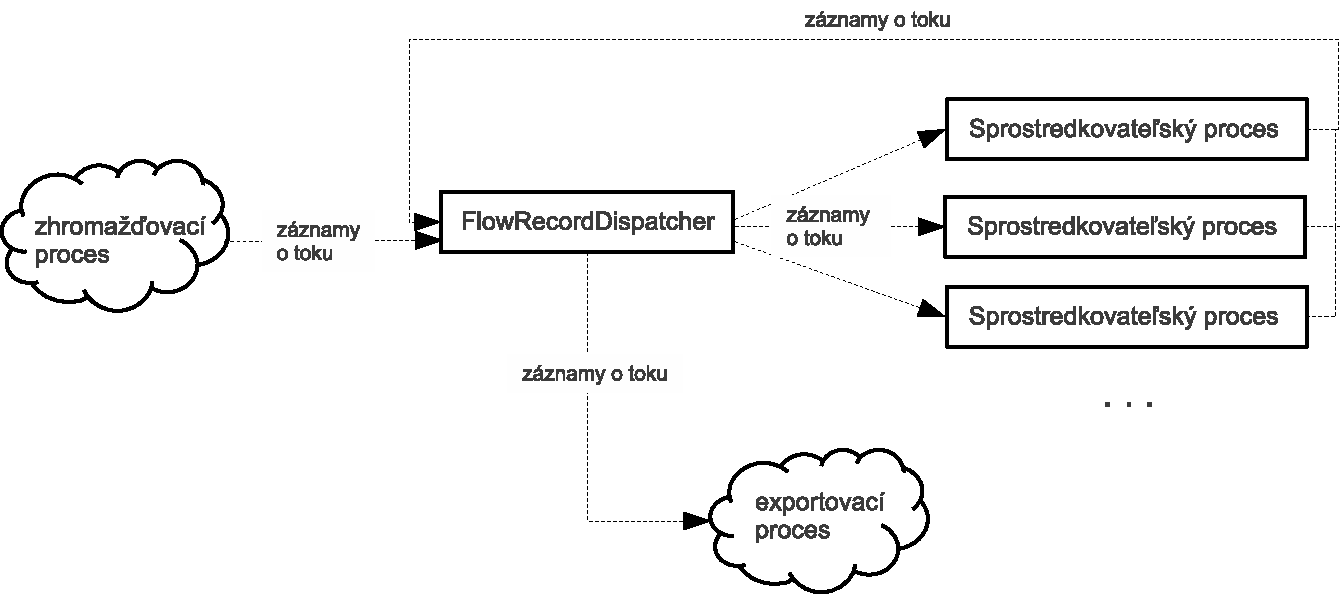
\includegraphics[width=0.9\textwidth]{flowRecordDispatcher_schema}
\caption{Schéma toku dát cez triedu FlowRecordDispatcher}\label{o:flowRecordDispatcher_schema}
\end{figure}

Úlohou tejto triedy je riadiť tok dát medzi komponentami IPFIX Mediátora na základe nastavenia
v~konfiguračnom súbore.
Ukážme si príklad takejto konfigurácie:
\begin{verbatim}
<processes>
        <process name="SelectionProcess">
            <input>exporter</input>
        </process>
        <process name="AggregationProcess">
            <input>exporter</input>
        </process>
        <process name="AnonymizationProcess">
            <input>AggregationProcess</input>
        </process>
</processes>
\end{verbatim}

Majme 3 sprostredkovateľské procesy: 
\begin{itemize}
\item SelectionProcess,
\item AggregationProcess a 
\item AnonymizationProcess.
\end{itemize}

Formát zápisu toku dát medzi procesmi je rovnaký ako v~príklade. Vstupnými údajmi pre 
\emph{SelectionProcess} a \emph{AggregationProcess} sú dáta priamo prijaté od exportéra, teda sú 
vlastne výstupom  
zhromažďovacieho procesu. Pričom vstupnými údajmi pre \emph{AnonymizationProcess} je výstup 
z~\emph{AggregationProcess}. Tie procesy, ktorých dáta nevstupujú do žiadneho iného sprostredkovateľského 
procesu sú logicky \uv{koncovými} procesmi, ich výstup je posunutý exportovaciemu procesu a poslaný 
kolektoru. Kým pri \emph{SelectionProcess} a \emph{AggregationProcess} hovoríme o~paralelnom spracovaní, 
\emph{AnonymizationProcess} spracováva záznamy sériovo.

Úloha triedy \verb|FlowRecordDispatcher| začína keď prijme prvé dáta od zhromažďovacieho procesu. Dáta prijíma 
cez nasledujúce dva 
parametre: záznam o~toku -- \verb|IPFIXFlowRecord| a reťazec určujúci odkiaľ tento záznam vystupuje -- 
\emph{inputProcess}.
Následne získa zoznam prijímateľov tohto záznamu o~toku, teda tie sprostredkovateľské procesy, 
ktorých položkou \emph{$<$input$>$} v~konfiguračnom súbore je reťazec \emph{inputProcess}, v~tomto 
prípade \uv{exporter}. Pri konfigurácii ako je daná v~príklade by zoznam obsahoval dva reťazce: 
\uv{SelectionProcess} a \uv{AggregationProcess}. Teraz potrebujeme získať inštancie týchto tried a ich 
vstupným vyrovnávacím pamätiam poslať 
prijatý záznam o~toku. FlowRecordDispatcher to vykoná v~cykle. 
Metódou \emph{getInstance(String processName)} zavolanou nad
abstraktnou triedou \emph{AIntermediateProcess} získa jedinú inštanciu sprostredkovateľského procesu. 
Tato metóda nie je triviálna, podrobne sme sa jej venovali v~Sekcii~\ref{sec:singleton} --
\emph{Jediná inštancia modulov}. Každej takto získanej 
inštancii sprostredkovateľského procesu zapíše do vstupnej pamäte -- \emph{inputBuffer} záznam o~toku.

Vstupnú vyrovnávaciu pamäť implementuje trieda \verb|IPInputBuffer|, ktorá je analógiou k~triede \verb|PacketCache|.
Samotnú pamäť rovnako predstavuje synchronizovaný a vysoko výkonný \emph{FIFO} front, implementovaný 
pomocou \verb|ArrayBlockingQueue|, do ktorého sú zapisované objekty typu \verb|IPFIXFlowRecord|.

Sú tri základne metódy s~rôznymi parametrami, ktoré zapisujú do frontu.
Metóda \emph{offer()} vloží objekt na koniec frontu, iba v~prípade, že je to možné 
okamžite bez prevýšenia kapacity frontu a vráti \emph{true} ak bol zápis úspešný, \emph{false}
v~opačnom prípade. Tato metóda sa viac preferuje ako \emph{add()}, ktorá pri neúspešnom zápise 
vyhodí výnimku. Treťou je metóda \emph{put()}. Jej špecialitou je to, že v~prípade, že je front plný,
čaká na uvoľnenie miesta. Toto však spôsobí zablokovanie celého vlákna \citep{arrayblockingqueue}.

V~zhromažďovacom procese, v~Kapitole~\ref{sec:navrh} (Sekcia~\ref{sec:collectingprocess}),
sa do frontu zapisuje metódou \emph{put()}. V~prípade, že sa \emph{PacketCache} naplní, je na mieste 
zablokovať \emph{UDPServer} a~počkať a uvoľnenie miesta vo vyrovnávacej pamäti. Avšak na tomto mieste by 
to nebolo vhodné. Stačilo by, že by jeden sprostredkovateľský proces nestíhal spracovávať svoje záznamy
o~tokoch, zablokovalo by to dispečera tokov a tým cele vlákno predstavujúce druhú fázu zhromažďovacieho
procesu. Kvôli jednému procesu by žiaden proces nedostával nové záznamy. Preto zápis do vstupnej pamäte
sprostredkovateľských procesov zabezpečuje metóda \emph{offer()}.

Ak metóda na získanie zoznamu prijímateľov vráti prázdny zoznam, znamená to, že~záznam o~toku 
sa nemá presmerovať ďalšiemu sprostredkovateľskému procesu, ale je už určený na export. Preto záznam
o~toku je zapísaný do vyrovnávacej pamäte pre export. Výsledkom je, že dáta boli presmerované správnym 
prijímateľom a boli splnené príslušné požiadavky na rámec pre IPFIX Mediátor.

%% ----------- FLOWRECORD DISPATCHER END ---------
%% -------------------- EXPORTING -----------------
\subsection{Exportovací proces}

Poslednou fázou Mediátora je exportovací proces. Jeho schéma je zobrazená na 
Obrázku~\ref{o:exporting_schema}. Ako bolo spomenuté v~predchádzajúcej kapitole, záznamy 
o~tokoch, ktoré sú výstupom \uv{koncových} sprostredkovateľských procesov sú prostredníctvom dispečera 
tokov pripravené na export zapísaním do exportovacej pamäte.

\begin{figure}[ht!]
\centering
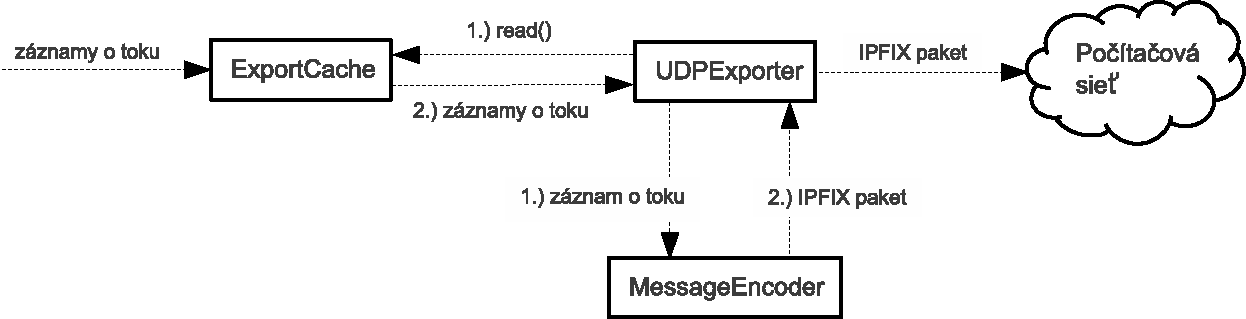
\includegraphics[width=0.8\textwidth]{exporting_schema}
\caption{Schéma exportovacieho procesu}\label{o:exporting_schema}
\end{figure}

Exportovaciu pamäť predstavuje \verb|ExportCache|. Tá je rovnako ako \verb|PacketCache| 
a~\verb|IPInputBuffer| synchronizovaný \emph{FIFO} front, do ktorého sa zapisujú objekty typu 
\verb|IPFIXFlowRecord|. Ak sa \verb|ExportCache| naplní, sprostredkovateľské procesy nemajú byť blokované, 
ale majú pokračovať vo svojej práci. Preto sa do frontu zapisuje metódou \emph{offer()}.

Jadrom exportovacieho procesu je trieda \verb|UDPExporter|, predstavujúca samostatné vlákno.
V~konštruktori vytvára UDP socket na prijímanie a posielanie paketov a~naviaže ho na akýkoľvek voľný port.
K~tomu slúži volanie bezparametrického konštruktora triedy \verb|DatagramSocket|. V~jeho hlavnej metóde 
\emph{run()} vykonáva cyklus dokiaľ nie je prerušený. V~cykle číta a vyberá záznamy o~tokoch
z~vyrovnávacej pamäte pre export. Záznamy posiela triede \verb|MessageEncoder|, ktorá z~neho poskladá 
IPFIX paket.

\verb|MessageEncoder| vo svojich metódach postupne tvori obsah IPFIX správy podľa formátu, ktorý bol 
analyzovaný v~Kapitole~\ref{sec:analyza} (Sekcia~\ref{sec:message_format}). Najprv vypočíta 
sekvenčné číslo, ktoré je obsahom hlavičky každej správy. Toto číslo zodpovedá celkovému počtu doteraz 
odoslaných dátových záznamov modulo $2^{32}$. Ich celkový počet si priebežne zvyšuje vo svojej členskej 
premennej. Potom postupne kóduje sady šablón, dátové sady, určí, resp. vypočíta všetky položky 
hlavičky správy a napokon všetko pospája do výslednej správy.

Trieda rozhoduje, či v~posielanej IPFIX správe má byť zahrnutá aj šablóna prislúchajúca dátovým záznamom
obsiahnutým v~zázname o~toku z~ktorého vytvára správu. Každá šablóna vo svojej členskej premennej uchováva
čas, kedy bola posledne exportovaná. Ak rozdiel medzi prítomnosťou a časom posledného exportu je väčší ako 
je hodnota \verb|<ipfixTemplateTimeout>| definovaná v~konfiguračnom súbore, tak šablóna musí byť pripojená.
Rovnako je šablóna pripojená okamžite po jej aktualizácii exportérom. 

Metóda na zakódovanie šablóny používa objekt triedy \verb|ByteArrayOutputStream|. Táto trieda 
implementuje prúd údajov, v~ktorom sú dáta zapisované do poľa bajtov. Do tohto prúdu postupne kóduje údaje 
v~takom poradí ako definuje formát IPFIX správy. Najprv do prúdu zakóduje číslo šablóny, za ním 
počet špecifikátorov poľa a potom samotné špecifikátory. Formát špecifikátorov je nasledovný. Ako prvé sa 
kóduje číslo informačného elementu na dvoch bajtoch. V~prípade, že ide o~element definovaný 
organizáciou, tak najvyšší bit sa nastaví na 1. Nasleduje dĺžka informačného elementu a v~prípade potreby 
číslo organizácie definované spoločnosťou IANA. Keď je prúd záznamu šablóny hotový, tak sa pred neho 
zaradia zakódované údaje sady šablóny. Tie pozostávajú z~čísla sady, čo je v~prípade sady šablóny číslo 2
a celkovej dĺžky záznamu šablóny 
vrátane veľkosti hlavičky sady. Touto operáciou vznikne prúd bajtov sady šablóny.

Po zakódovaní šablóny sa postupne kódujú všetky dátové záznamy obsiahnuté v~zázname toku. Jednotlivé 
hodnoty polí už sú správne zakódované podľa dátového typu, toto majú na zodpovednosti sprostredkovateľské
procesy. Takže v~tejto fáze stačí cyklicky prejsť všetky dátové záznamy a ich zakódované polia zapísať 
do prúdu bajtov. Napokon je potrebné pred tento prúd zaradiť zakódované údaje dátovej sady. Konkrétne
ide o~číslo prislúchajúcej šablóny a súčet dĺžok všetkých dátových záznamov vrátane veľkosti hlavičky sady.
Takto je vytvorený prúd bajtov dátovej sady.

Ako posledný sa zostaví prúd bajtov hlavičky IPFIX správy. Dĺžka správy je určená súčtom veľkosti hlavičky
správy s~veľkosťou sady šablóny a dátovej sady. Ako prvé sa do prúdu bajtov hlavičky zakóduje číslo 
verzie, teda \verb|0x000a| a dĺžka správy. Nasleduje čas exportu, vypočítané sekvenčné číslo a ID 
pozorovacej domény, ktoré je nastavené administrátorom v~konfiguračnom súbore. Toto číslo však definuje
pozorovaciu doménu v~ktorej sídli Mediátor, nie exportér. O~určovaní času exportu podrobnejšie neskôr.

V~analýze boli uvedené implementačno-špecifické problémy Mediátora, Kapitola~\ref{sec:analyza} 
(Sekcia~\ref{sec:problems}). Prvým bola strata informácii o~pôvodnom exportéri. Ako bolo spomenuté neskôr, 
v~analýze exportovacieho procesu v~Kapitole~\ref{sec:analyza} (Sekcia~\ref{sec:exporting_process}),
spôsobom ako posielať tieto informácie je zakódovať ich do informačných elementov skupiny 2. Na požiadavku
Mediátora boli všetky informačné elementy z~Tabuľky \ref{t:ie-group2} implementované na strane exportéra.
ID pozorovacieho bodu a pozorovacej domény v~ktorej sídli exportér sa kolektor dozvie z~príslušných 
informačných elementov, ktoré taktiež exportér podporuje. 

Druhým problémom bola strata informácie o~čase exportu. RFC 6183 \citep{rfc6183} popisuje dva spôsoby 
určenia času exportu:
\begin{enumerate}
 \item Zachovávať hodnotu z~hlavičky prichádzajúcich IPFIX správ.
 \item Nastaviť aktuálnu hodnotu času keď IPFIX správa opúšťa Mediátor.
\end{enumerate}
V~prípade, že exportér posiela akýkoľvek \uv{\emph{delta}} informačný element, napr. \emph{flowStartDeltaMicroseconds},
tak musí byť použitý prvý spôsob určenia času exportu, teda zachovanie pôvodného času. Keďže 
\uv{\emph{delta}} hodnoty sa viažu na tento čas, pri jeho prepísaní by stratili význam. Aby Mediátor 
vyhovoval obom prípadom, navrhli sme, že spôsob určovania času exportu definuje administrátor
v~konfiguračnom súbore, v~elemente \verb|<exportTime>|. 
Ak zadá reťazec \verb|KEEP|, tak trieda \verb|MessageEncoder| zakóduje do prúdu bajtov hlavičky pôvodnú
hodnotu. V~prípade reťazca \verb|RENEW| sa zakóduje aktuálna hodnota času.

Poslednou úlohou triedy \verb|MessageEncoder| je pospájať jednotlivé prúdy bajtov do výsledného prúdu IPFIX 
správy. Prvým je prúd bajtov hlavičky správy. Ak sa exportuje aj šablóna, tak nasleduje prúd sady šablóny 
a posledným je prúd dátovej sady. Trieda \verb|UDPExporter| teraz z~prúdu IPFIX správy vytvorí 
UDP paket. Na to slúži trieda \verb|DatagramPacket|, pričom jej parametrami sú dáta, dĺžka správy, 
IP adresa a UDP port. Posledné dve menované sú zadané administrátorom v~konfiguračnom súbore. Metódou 
\emph{send()} zavolanou nad socketom je správa odoslaná.







%
\section{Experimentálne overenie funkčnosti riešenia}

Tato kapitola je venovaná overeniu správnosti implementácie. Boli vykonané nasledujúce štyri experimenty, 
ktoré mali potvrdiť, alebo vyvrátiť správnu funkčnosť riešenia. 
\begin{enumerate}
 \item \textbf{Prvý test} overil konektivitu a prenos údajov medzi exportérom a mediátorom a následne medzi 
 mediátorom a kolektorom.
 \item \textbf{Druhy test} porovnal hodnoty údajov exportovaných mybeem-om s hodnotami uloženými v databáze po prechode
 cez Mediátor bez sprostredkovateľského procesu.
 \item \textbf{Tretí test} demonštroval správnosť anonymizácie údajov v podaní sprostredkovateľského procesu 
 \verb|ExampleProcess|, spomínaného vyššie v návrhu a implementácii.
 \item \textbf{Štvrtý test} bol tzv. záťažovým testom, overoval stabilitu Mediátora pri dlhodobom behu a 
 pri spracovávaní prevádzky s vysokým počtom tokov.
\end{enumerate}

%%%%%

\subsection{Testovacia topológia}

Pri všetkých testoch bol použitý virtualizačný nástroj VirtualBox, v ktorom boli vytvorené tri virtuálne 
počítače, zapojené do topológie, ktorú možno vidieť na Obrázku \ref{o:test_topologia}.
Na všetkých troch počítačoch sa používal operačný systém Ubuntu 12.04 LTS v desktopovej verzii. Na prvom 
počítači bol nainštalovaný exportér mybeem (verzia 1.1-6 s podporou pre IPFIX Mediátor), ktorý exportoval 
správy druhému počítaču na UDP port vyhradený pre IPFIX komunikáciu - \emph{4739}. Tam bežal Mediátor
verzie 1.0. Ten zase preposielal správy na tretí počítač (taktiež port \emph{4739}), kde bol spustený 
kolektor JXColl (verzia 3.9) s funkčnou PostgreSQL databázou. Počítače boli zapojené v jednej lokálnej 
sieti a všetky mali prístup na Internet.

\begin{figure}[ht!]
\centering
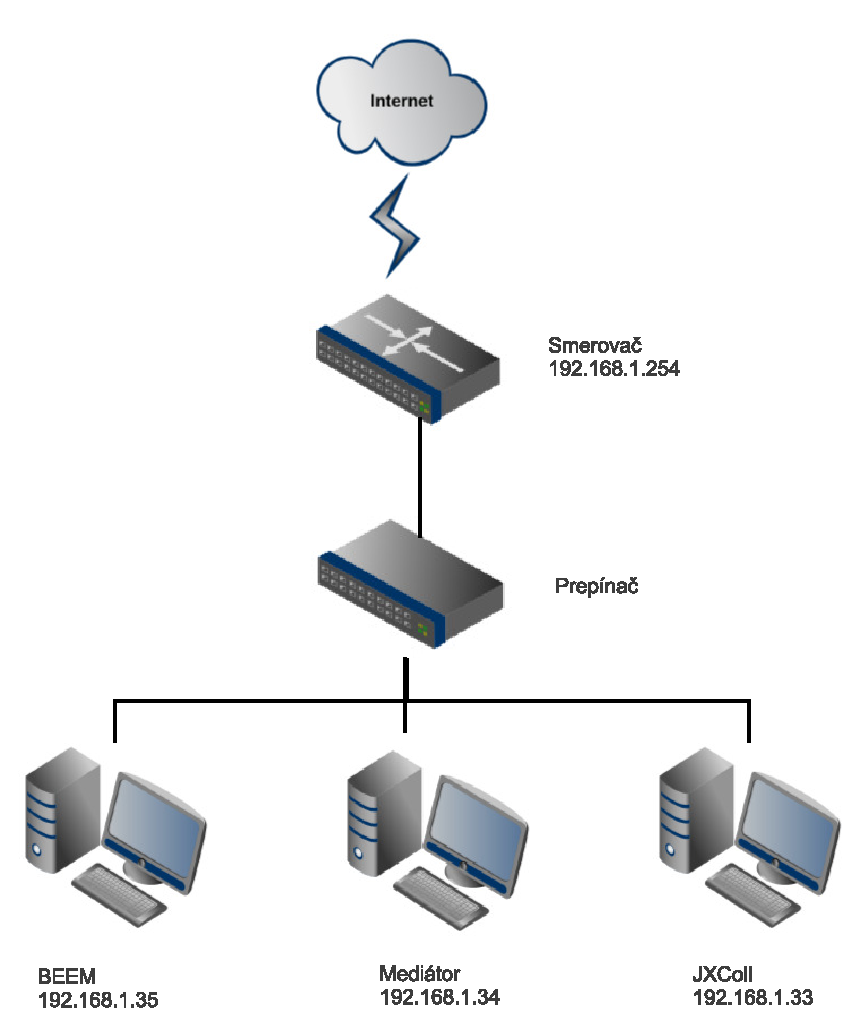
\includegraphics[width=0.8\textwidth]{test_topologia}
\caption{Testovacia topológia}\label{o:test_topologia}
\end{figure}

%%-------------------------

\subsection{Test konektivity}

Prvý experiment overoval základnú konektivitu medzi exportérom a kolektorom v prípade, že je medzi ne 
zaradený mediátor. Vo svojej východiskovej konfigurácii vypisuje mybeem logovacie správy na štandardný 
výstup. Tie obsahujú základné informácie o každom exportovanom zázname o toku ako to môžeme vidieť na 
Obrázku \ref{o:konektivita_beem}. Mediátor mal nastavenú úroveň logovacích výstupov na \emph{DEBUG}, 
čo zahŕňa nielen chybové hlášky, ale aj všetky informačné a ladiace oznamy. 

Konektivita medzi exportérom
a mediátorom bola potvrdená, na Obrázku \ref{o:konektivita_mediator} je zachytený výstup Mediátora po 
prijatí správy od exportéra. Výpis obsahuje IP adresu a port z ktorého prišla správa, jej veľkosť a 
oznam, že ide o IPFIX správu. Za tým nasledujú hodnoty z hlavičky správy a výpis všetkých sád, ktoré
správa obsahuje. Potom bol spracovaný záznam o toku posunutý dispečerovi - \verb|FlowRecordDispatcher|, 
ktorý ho poslal na export. Tam sa záznam o toku naspať zabalil do nového IPFIX paketu a ten bol odoslaný 
smerom na kolektor.

\begin{figure}[ht!]
\centering
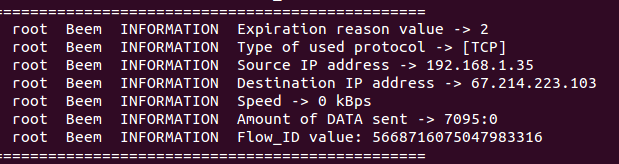
\includegraphics[width=0.9\textwidth]{konektivita_beem}
\caption{Test 1: Konektivita medzi exportérom a Mediátorom - strana exportéra}\label{o:konektivita_beem}
\end{figure}

\begin{figure}[ht!]
\centering
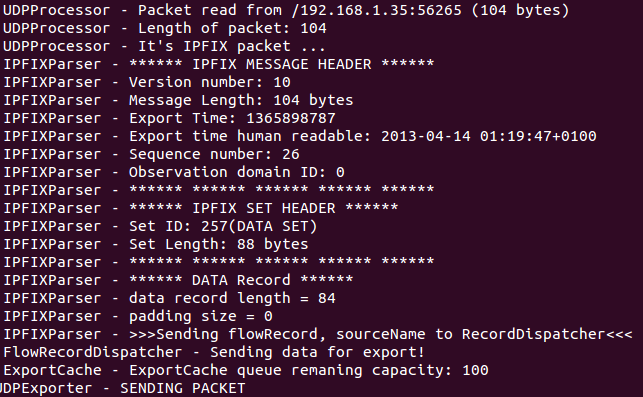
\includegraphics[width=0.9\textwidth]{konektivita_mediator}
\caption{Test 1: Konektivita medzi exportérom a Mediátorom - strana Mediátora}\label{o:konektivita_mediator}
\end{figure}

Konektivita medzi Mediátorom a kolektorom bola tiež potvrdená. Dôkazom boli logovacie výstupy kolektora, 
ktoré sú veľmi podobné ako tie z Mediátora. V databáze, na ktorú je JXColl pripojený, pribúdali správne 
záznamy. Tento experiment môžeme považovať za úspešný.

%%-------------------------

\subsection{Test správnej reprezentácie údajov}

Druhý experiment nadväzoval na predchádzajúci test konektivity. Testovacia topológia aj konfigurácie 
jednotlivých nástrojov boli rovnaké ako v predchádzajúcom prípade. V Mediátore stále neboli spustené 
žiadne sprostredkovateľské moduly. 

\begin{figure}[ht!]
\centering
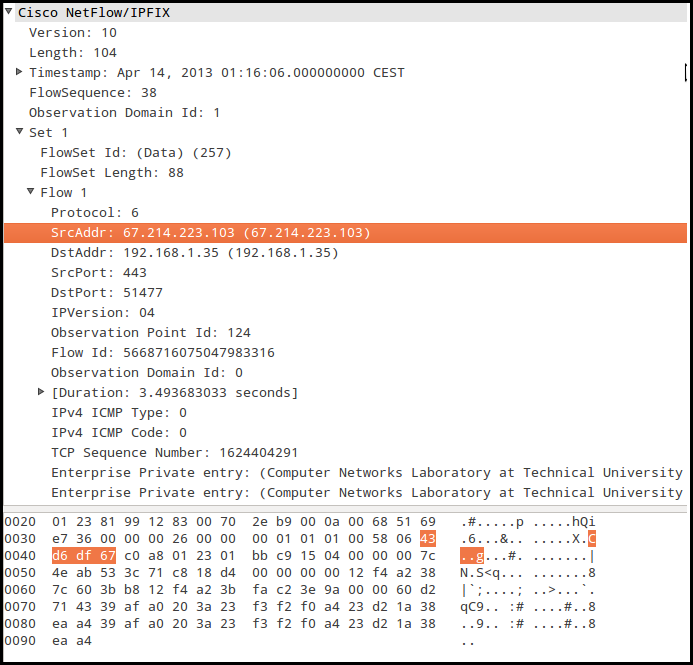
\includegraphics[width=1.0\textwidth]{porovnanie_wireshark}
\caption{Test 2: Správy odosielané exportérom zachytené programom Wireshark}\label{o:porovnanie_wireshark}
\end{figure}

\begin{figure}[ht!]
\centering
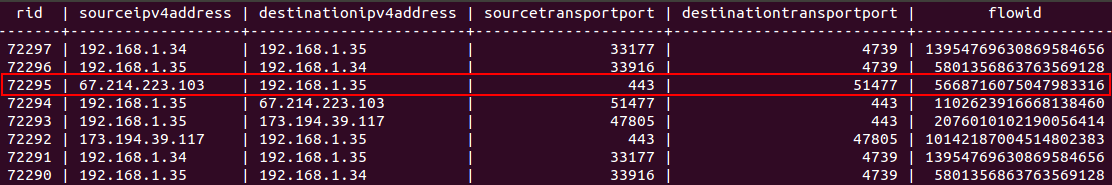
\includegraphics[width=1.0\textwidth]{porovnanie_db}
\caption{Test 2: Výpis obsahu databázy}\label{o:porovnanie_db}
\end{figure}

Myšlienkou tohto overenia bolo porovnať dáta, ktoré posiela exportér s dátami, ktoré prejdú celou topológiou
cez Mediátor a JXColl a sú uložené v databáze. Na zachytenie správ z mybeem-u bol použitý program 
Wireshark, ktorý odchytával sieťovú prevádzku na prvom počítači, na rozhraní \emph{eth0} s IP adresou 
\emph{192.168.1.35}. Detail jednej zo správ, ktoré zachytil Wireshark je na Obrázku 
\ref{o:porovnanie_wireshark}. Na Obrázku \ref{o:porovnanie_db} sú zase vyfiltrované posledné záznamy, 
ktoré boli uložené do databázy. Môžeme porovnať aspoň na niekoľkých znázornených informačných elementoch,
že záznamy o toku sa po prechode cez topológiu s Mediátorom bez zapnutých sprostredkovateľských procesov 
nezmenili. Tento experiment považujeme za úspešný.

%%-------------------------

\subsection{Test Mediátora s anonymizačným modulom}

Tento experiment je miernou úpravou predchádzajúceho. Testovacia topológia aj konfigurácie nástrojov boli 
rovnaké s tým rozdielom, že v Mediátore bol zapnutý jednoduchý anonymizačný proces - \verb|ExampleProcess|.
Tento modul bol naprogramovaný kvôli demonštrácii implementácie sprostredkovateľského procesu. Cieľom 
experimentu bolo dokázať dve tvrdenia:
\begin{itemize}
 \item Aplikačný rámec poskytuje sprostredkovateľským procesom správne metódy na dekódovanie a zakódovanie
 dátových záznamov. To platí vtedy, keď hodnoty informačných elementov sa rovnajú hodnotám záznamov
 v databáze po prechode celou topológiou aj keď sú spustené sprostredkovateľské moduly.
 \item Anonymizačný modul správne modifikuje zdrojovú a cieľovú IP adresu toku. Výsledkom je to, že 
 posledný oktet je v obidvoch prípadoch nahradený nulou.
\end{itemize}

\begin{figure}[ht!]
\centering
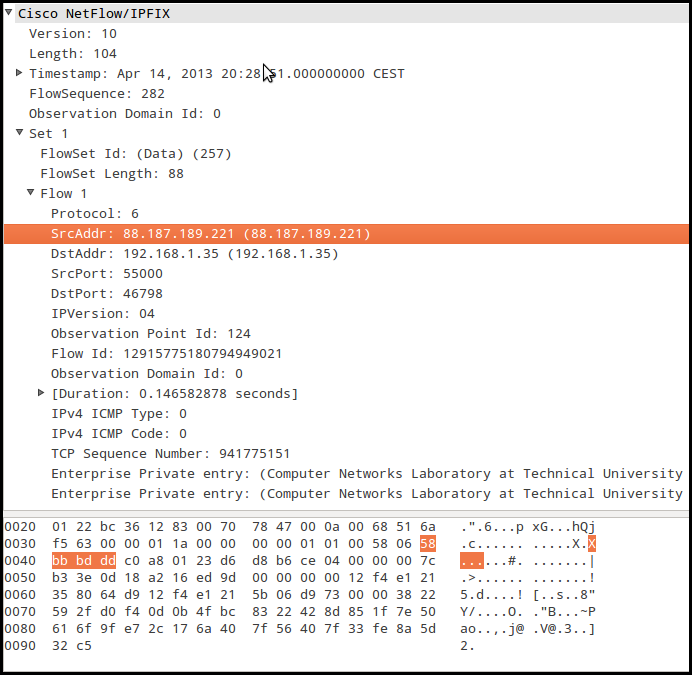
\includegraphics[width=1.0\textwidth]{anonym_wireshark}
\caption{Test 3: Správy odosielané exportérom zachytené programom Wireshark}\label{o:anonym_wireshark}
\end{figure}

\begin{figure}[ht!]
\centering
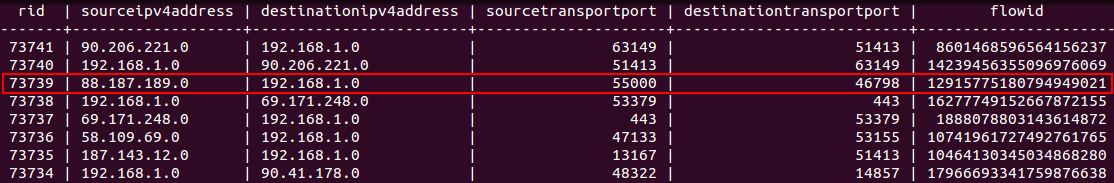
\includegraphics[width=1.0\textwidth]{anonym_db}
\caption{Test 3: Výpis obsahu databázy}\label{o:anonym_db}
\end{figure}


Na Obrázku \ref{o:anonym_wireshark} je zobrazený detail jednej zo správ, ktorú exportoval mybeem. 
Na nasledujúcom Obrázku \ref{o:anonym_db} vidieť posledne záznamy z databázy. Môžeme porovnať, že hodnoty 
zdrojového a cieľového transportného portu a hodnota \emph{flowId} sa nezmenili. Avšak zároveň, všetky 
zdrojové a cieľové IP adresy boli anonymizované. Tento experiment považujeme za úspešný, dokázal správnosť 
obidvoch tvrdení.


\subsection{Záťažový test}






%
\section{Zhodnotenie rie\v{s}enia}

Najdôležitejším cieľom tejto diplomovej práce bolo navrhnúť a implementovať aplikačný rámec pre 
sprostredkovateľskú entitu (IPFIX Mediátor), ktorá by bola medzičlánkom v komunikácii medzi exportérom
BEEM a kolektorom JXColl nástroja SLAmeter. Mediátor má poskytovať rozhranie pre manipuláciu so 
sprostredkovateľskými modulmi, ktoré budú poskytovať rôzne funkcie na modifikáciu IPFIX správ ešte pred ich 
spracovaním v kolektore. Práca túto úlohu aj splnila, čo bolo potvrdené v poslednej časti 
práce venovanej experimentálnemu overeniu.

Úvodom sa čitateľ oboznámil s analýzou formátu IPFIX správ rovnako ako s výhodami použitia 
IPFIX Mediátora v meracej architektúre. Samostatné časti boli venované príkladom použitia, ale aj 
úskaliam spojeným s implementáciou tohto nástroja. Nechýbalo ani stručné predstavenie projektov výskumnej 
skupiny MONICA.

Najvýznamnejším výsledkom práce je funkčná implementácia aplikačného rámca v jazyku Java. Jeho návrh je 
odpoveďou na definované požiadavky a analyzované implementačno-špecifické problémy. Zhromažďovací proces 
bol prispôsobený, no vychádzal z existujúcej implementácie kolektoru JXColl. Dôležitou častou práce je 
podpora pre sprostredkovateľské procesy. Tok dát medzi modulmi, či už sériový, alebo paralelný sa  
jednoducho nastavuje v konfiguračnom XML súbore podľa navrhnutého formátu. Na základe tejto konfigurácie 
riadi dispečer distribúciu záznamov o tokoch medzi procesmi. Definované moduly sa však najprv musia 
pospúšťať. Toto zabezpečila pokročilá technológia dynamického načítavania tried pomocou 
systémového \emph{class loadera} a reflexie. Ďalším pokročilým riešením bolo zabezpečenie toho, že 
všetky sprostredkovateľské moduly musia mať len jednu unikátnu inštanciu. Keďže dizajn jazyka Java 
nepovoľuje \emph{abstract static} metódy, bolo potrebné využiť návrhový vzor \emph{Factory method} a 
hash mapu uchovávajúcu existujúce inštancie modulov. 

Úlohou aplikačného rámca je aj poskytnúť metódy na dekódovanie a zakódovanie hodnôt informačných elementov.
Pri zakódovaní bol kladený veľký doraz na efektivitu a výpočtový výkon. Preto navrhnuté metódy namiesto 
využívania tried jazyka pracujú na úrovni bitových operácii. Budúci riešitelia určite ocenia prítomnosť
vzorového sprostredkovateľského modulu, ktorý demonštruje navrhnuté zásady programovania modulov a 
využíva všetky dostupné metódy, ktoré mu poskytuje abstraktná rodičovská trieda. 

Implementácia bola nakoniec overená niekoľkými experimentmi, ktoré dokázali funkčnosť riešenia. Ďalšie 
smerovanie nástroja predpokladá implementovanie sprostredkovateľských modulov, ktoré zlepšia monitorovacie 
možnosti aplikácie SLAmeter. Najväčší prínos sa vidí v anonymizačnom module, konverznom module z protokolu 
NetFlow na IPFIX, prípadne v module, ktorý
bude na základe istých pravidiel robiť selekciu IPFIX správ a tie následne exportovať distribuovaným 
kolektorom. Z pohľadu aplikačného rámca by bolo vhodné rozšíriť jeho zhromažďovací proces o podporu 
ďalších transportných protokolov ako TCP a SCTP. Rovnaké rozšírenie je možné aj na strane exportovacieho 
procesu.


%Táto časť\/ záverečnej práce je povinná. Autor uvedie zhodnotenie
%riešenia. Uvedie výhody, nevýhody riešenia,  použitie výsledkov, ďalšie
%možnosti a~pod., prípadne načrtne iný spôsob riešenia úloh, resp.
%uvedie, prečo postupoval uvedeným spôsobom.
%
%%
\begin{thebibliography}{999}
\addcontentsline{toc}{section}{\numberline{}Zoznam pou\v{z}itej
literat\'ury}

%----------- RFC ------------------------

\harvarditem{Information Sciences Institute}{1981}{rfc791}
Information Sciences Institute, University of Southern California: \emph{Internet protocol} 
RFC 791. 1981

\harvarditem{Deering, Hinden}{1998}{rfc2460}
DEERING, S., HINDEN, R.: \emph{Internet Protocol, Version 6 (IPv6) - Specification} 
RFC 2460. 1998

\harvarditem{Claise et al.}{2008}{rfc5101}
CLAISE, B. et al.: \emph{Specification of the IP Flow Information Export 
(IPFIX) Protocol for the Exchange of IP Traffic Flow Information.} 
RFC 5101. 2008

\harvarditem{Quittek, et al.}{2008}{rfc5102}
QUITTEK, J. et al.: \emph{Information Model for IP Flow Information Export} 
RFC 5102. 2008

\harvarditem{Quittek et al.}{2004}{rfc3917}
QUITTEK, J. et al.: \emph{Requirements for IP Flow Information Export (IPFIX).} 
RFC 3917. 2004

\harvarditem{Kobayashi, Claise}{2010}{rfc5982}
KOBAYASHI, A. -- CLAISE, B. et al.: \emph{IP Flow Information Export (IPFIX) Mediation: Problem Statement.} 
RFC 5982. 2010

\harvarditem{Kobayashi et al.}{2011}{rfc6183}
KOBAYASHI, A. et al.: \emph{IP Flow Information Export (IPFIX) Mediation: Framework.} 
RFC 6183. 2011

\harvarditem{Claise}{2004}{rfc3954}
CLAISE, B.: \emph{Cisco Systems NetFlow Services Export Version 9.} 
RFC 3954. 2004

\harvarditem{Mills}{1992}{rfc1305}
MILLS, D. L.: \emph{Network Time Protocol (Version 3) Specification, Implementation and Analysis.} 
RFC 1305. 1992

\harvarditem{Zseby, et al.}{2009}{rfc5475}
ZSEBY, T. et al.: \emph{Sampling and Filtering Techniques for IP Packet Selection} 
RFC 5475. 2009

\harvarditem{Sadasivan, et al.}{2009}{rfc5470}
SADASIVAN, G. et al.: \emph{Architecture for IP Flow Information Export} 
RFC 5470. 2009

%-----------------------------------

\harvarditem{IPFIX charter}{2013}{ipfixCharter}
The IPFIX Charter: \emph{IP Flow Information Export (ipfix)} [online], 2013. Dostupné 
z: $<$\url{http://www.ietf.org/html.charters/ipfix-charter.html}$>$.

\harvarditem{IPFIX protocol}{}{ipfixProtocol}
Javvin network management \& security: \emph{IPFIX: Internet Protocol Flow Information eXport} [online]. Dostupné 
z: $<$\url{http://www.javvin.com/protocolIPFIX.html}$>$.

\harvarditem{Juvhaugen}{2007}{juvhaugen}
JUVHAUGEN, P.: \emph{Exporting IP flows using IPFIX.} 
Diplomová práca. Oslo: Oslo University College FI, 2007. 18 s. Dostupné 
z: $<$\url{http://hdl.handle.net/10642/434}$>$.

\harvarditem{Vereščák}{2012}{veri}
VEREŠČÁK, T.: \emph{Optimalizácia zhromažďovacieho procesu nástroja BasicMeter.} 
Diplomová práca. Košice: Technická univerzita. Fakulta elektrotechniky a informatiky. 
Katedra počítačov a informatiky, 2012.

\harvarditem{Private Enterprise Numbers}{2013}{pen}
IANA: \emph{Private Enterprise Numbers} [online], 2013. Dostupné 
z: $<$\url{http://www.iana.org/assignments/enterprise-numbers}$>$.

\harvarditem{Cho et. al}{2006}{trafgrw}
CHO, K., FUKUDA, K., ESAKI, H., KATO, A.: \emph{The Impact and Implications of the Growth in Residential
User-to-User Traffic}, SIGCOMM2006, pp. 207-218, Pisa, Taliansko, September 2006.

\harvarditem{IEEE 802.3ad}{2000}{ieee802.3}
IEEE Computer Society: \emph{Link Aggregation}, IEEE Std 802.3ad-2000, March 2000.

\harvarditem{Pekár}{2009}{ado}
PEKÁR, A.: \emph{Monitorovanie prevádzkových parametrov siete v reálnom čase.} 
Bakalárska práca. Košice: Technická univerzita. Fakulta elektrotechniky a informatiky. 
Katedra počítačov a informatiky, 2009.

\harvarditem{MONICA}{2013}{monica}
Výskumná skupina MONICA: \emph{Nástroj BasicMeter} [online], 2013. 
Dostupné z: $<$\url{http://wiki.cnl.sk/Monica/BasicMeter}$>$.

\harvarditem{Kudla}{2010}{ja}
KUDLA, R.: \emph{Experimentálne prostredie pre nástroj BasicMeter.} 
Bakalárska práca. Košice: Technická univerzita. Fakulta elektrotechniky a informatiky. 
Katedra počítačov a informatiky, 2010.

\harvarditem{SLAmeter}{2013}{slameter}
Výskumná skupina MONICA: \emph{SLAmeter} [online], 2013. 
Dostupné z: $<$\url{http://wiki.cnl.sk/Monica/SLAmeter}$>$.

\harvarditem{Vyhodnocovač}{2013}{evaluator}
Výskumná skupina MONICA: \emph{Vyhodnocovač} [online], 2013. 
Dostupné z: $<$\url{http://wiki.cnl.sk/Monica/VyhodnocovacSLA}$>$.

%--------------------JAVA ------------------------------------
\harvarditem{Mcmanis}{1996}{mcmanis}
MCMANIS, CH.: \emph{The basics of Java class loaders} [online], 1996. Dostupné 
z: $<$\url{http://www.javaworld.com/javaworld/jw-10-1996/jw-10-indepth.html}$>$.

\harvarditem{Travis}{2001}{travis}
TRAVIS, G.: \emph{Understanding the Java ClassLoader} [online], 2001. Dostupné 
z: $<$\url{http://www.ibm.com/developerworks/java/tutorials/j-classloader}$>$.

\harvarditem{TechJava}{2008}{techjava}
TechJava: \emph{Java Class Loading} [online], 2008. Dostupné 
z: $<$\url{http://www.techjava.de/topics/2008/01/java-class-loading/}$>$.

\harvarditem{Antl}{2012}{antl}
ANTL, M.: \emph{Rámec vyhodnocovača a webového rozhrania nástroja SLA Meter} 
Diplomová práca. Košice: Technická univerzita. Fakulta elektrotechniky a informatiky. 
Katedra počítačov a informatiky, 2012.

\harvarditem{Christudas}{2005}{christudas}
CHRISTUDAS, B.: \emph{Internals of Java Class Loading} [online], 2005. Dostupné 
z: $<$\url{http://www.onjava.com/pub/a/onjava/2005/01/26/classloading.html}$>$.

\harvarditem{Oracle}{2011}{classloader}
Oracle: \emph{Class ClassLoader} [online], Java 6 - oficiálna špecifikácia API, 2011. 
Dostupné z: $<$\url{http://docs.oracle.com/javase/6/docs/api/java/lang/ClassLoader.html}$>$.

\harvarditem{Gallagher}{2010}{gallagher}
GALLAGHER, N: \emph{Inherited Java Singleton Problem} [príspevok na diskusnom fóre], 2010. 
Dostupné z: $<$\url{http://c2.com/cgi/wiki?InheritedJavaSingletonProblem}$>$.

\harvarditem{Oracle}{2013}{java_spec}
Oracle: \emph{Java Language and Virtual Machine Specifications} [online], 2013. 
Dostupné z: $<$\url{http://docs.oracle.com/javase/specs/}$>$.

\harvarditem{Oracle}{2011}{arrayblockingqueue}
Oracle: \emph{Class ArrayBlockingQueue$<$E$>$} [online], Java 6 - oficiálna špecifikácia API, 2011. 
Dostupné z: 
$<$\url{http://docs.oracle.com/javase/6/docs/api/java/util/concurrent/ArrayBlockingQueue.html#offer(E)}$>$.

\harvarditem{BitTorrent.org}{2009}{bittorrent}
BitTorrent.org: \emph{The BitTorrent Protocol Specification} [online], 2009. 
Dostupné z: $<$\url{http://www.bittorrent.org/beps/bep_0003.html}$>$.

\end{thebibliography}
%
\section*{Zoznam pr\'iloh}
\addcontentsline{toc}{section}{\numberline{}Zoznam pr\'iloh}
\thispagestyle{empty}

\begin{description}
	\item[Príloha A] Systémová príručka Mediator v1.0
	\item[Príloha B] Používateľská príručka Mediator v1.0
	\item[Príloha C] CD médium obsahujúce:
		\subitem diplomovú prácu v~elektronickej podobe (PDF, \LaTeX)
		\subitem systémovú príručku Mediator v1.0 (PDF, \LaTeX)
		\subitem používateľskú príručku Mediator v1.0 (PDF, \LaTeX)
		\subitem zdrojové súbory Mediator v1.0 (Java)
		\subitem DEB inštalačný balík pre Mediator v1.0 (DEB)
\end{description}
%
\section*{Pr\'iloha A}
\addcontentsline{toc}{section}{\numberline{}Pr\'iloha A}
\subsection*{Pr\'ilohy}

Táto časť\/ záverečnej práce je povinná a~obsahuje zoznam všetkých
príloh vrátane elektronických nosičov. Názvy príloh v~zozname musia
byť\/ zhodné s~názvami uvedenými na príslušných prílohách. Tlačené
prílohy majú na prvej strane identifikačné údaje -- informácie zhodné
s~titulnou stranou záverečnej práce doplnené o~názov príslušnej
prílohy. Identifikačné údaje sú aj na priložených diskoch alebo
disketách. Ak je médií viac, sú označené aj číselne v~tvare $I/N$, kde
$I$ je poradové číslo a~$N$ je celkový počet daných médií. Zoznam
príloh má nasledujúci tvar:
\begin{description}
\item[Príloha A] CD médium -- záverečná práca v~elektronickej podobe,
prílohy v~elektronickej podobe.
\item[Príloha B] Používateľská príručka
\item[Príloha C] Systémová príručka
\end{description}
Prílohová časť\/ je samostatnou časťou kvalifikačnej práce. Každá
príloha začína na novej strane a je označená samostatným písmenom
(Príloha A, Príloha B, \dots). Číslovanie strán príloh nadväzuje na
číslovanie strán v~hlavnom texte. Pri každej prílohe sa má uviesť\/
prameň, z~ktorého sme príslušný materiál získali.
%
\section*{Pr\'iloha B}
\addcontentsline{toc}{section}{\numberline{}Pr\'iloha B}
\subsection*{Bibliografick\'e odkazy}

Táto časť\/ záverečnej práce je povinná. V~zozname použitej literatúry
sa uvádzajú odkazy podľa normy STN~ISO~690--2 (01 0197) (Informácie
a~dokumentácia. Bibliografické citácie. Časť\/ 2: Elektronické
dokumenty alebo ich časti, dátum vydania 1.~12.~2001, ICS:~01.140.20).
Odkazy sa môžu týkať\/ knižných, časopiseckých a~iných zdrojov
informácií (zborníky z~konferencií, patentové dokumenty, normy,
odporúčania, kvalifikačné práce, osobná korešpondencia a~rukopisy,
odkazy cez sprostredkujúci zdroj, elektronické publikácie), ktoré boli
v~záverečnej práci použité.

Forma citácií sa zabezpečuje niektorou z~metód, opísaných v~norme
STN~ISO~690, 1998, s.~21. Podrobnejšie informácie nájdete na stránke
\texttt{http://www.tuke.sk/anta/} v~záložke {\small\sf Výsledky
práce/Prehľad normy pre publikovanie STN~ISO~690 a~STN~ISO~690-2}.

Existujú dva hlavné spôsoby citovania v~texte.

\begin{itemize}
\item Citovanie podľa mena a~dátumu.
\item Citovanie podľa odkazového čísla.
\end{itemize}

\emph{Preferovanou metódou citovania} v~texte vysokoškolskej
a~kvalifikačnej práce je podľa normy ISO~7144 citovanie podľa mena
a~dátumu \citep{kat,gonda}. V~tomto prípade sa zoznam použitej
literatúry upraví tak, že za meno sa pridá rok vydania. Na uľahčenie
vyhľadávania citácií sa zoznam vytvára v~abecednom poradí autorov.

\medskip

Príklad:
\dots podľa \citep{steinerova} je táto metóda dostatočne rozpracovaná
na to, aby mohla byť\/ všeobecne používaná v~\dots

\medskip

Druhý spôsob uvedenia odkazu na použitú literatúru je uvedenie len
čísla tohto zdroja v~hranatých zátvorkách bez mena autora (autorov)
najčastejšie na konci príslušnej vety alebo odstavca.

\medskip

Príklad:
\dots podľa [13] je táto metóda dostatočne rozpracovaná na to, aby
mohla byť\/ všeobecne používaná v~\dots ako je uvedené v~[14].

\medskip

Citácie sú spojené s~bibliografickým odkazom poradovým číslom v~tvare
indexu alebo čísla v~hranatých zátvorkách. Odkazy v~zozname na konci
práce budú usporiadané podľa týchto poradových čísel. Viacero citácií
toho istého diela bude mať\/ rovnaké číslo. Odporúča sa usporiadať\/
jednotlivé položky v~poradí citovania alebo podľa abecedy.

\medskip
\noindent
Rôzne spôsoby odkazov je možné dosiahnuť\/ zmenou voľby v~balíku
\verb+natbib+:

\noindent
\verb+% Citovanie podla mena autora a roku+\\
\verb+\usepackage[]{natbib}\citestyle{chicago}+\\
\verb+% Možnosť rôznych štýlov citácií. Príklady sú uvedené+\\
\verb+% v preambule súboru natbib.sty.+\\
\verb+% Napr. štýly chicago, egs, pass, anngeo, nlinproc produkujú+\\
\verb+% odkaz v tvare (Jones, 1961; Baker, 1952). V prípade, keď+\\
\verb+% neuvedieme štýl citácie (vynecháme \citestyle{}) v "options"+\\
\verb+% balíka natbib zapíšeme voľbu "colon".+

\medskip
\noindent
Keď zapneme voľbu \verb+numbers+, prepneme sa do režimu citovania
podľa odkazového čísla.

\noindent
\verb+% Metoda ciselnych citacii+\\
\verb+\usepackage[numbers]{natbib}+

\bigskip

Pri zápise odkazov sa používajú nasledujúce pravidlá:

V~odkaze na knižnú publikáciu (pozri príklad zoznamov na konci tejto
časti):
\begin{itemize}
\item Uvádzame jedno, dve alebo tri prvé mená oddelené pomlčkou,
ostatné vynecháme a~namiesto nich napíšeme skratku et al. alebo a~i.
\item Podnázov sa môže zapísať\/ vtedy, ak to uľahčí identifikáciu
dokumentu. Od názvu sa oddeľuje dvojbodkou a~medzerou.
\item Dlhý názov sa môže skrátiť\/ v~prípade, ak sa tým nestratí
podstatná informácia. Nikdy sa neskracuje začiatok názvu. Všetky
vynechávky treba označiť\/ znamienkami vypustenia  \uv{\dots}
\end{itemize}

Pri využívaní informácií z~elektronických dokumentov  treba
dodržiavať\/ tieto zásady:
\begin{itemize}
\item  uprednostňujeme autorizované súbory solídnych služieb
a~systémov,
\item zaznamenáme dostatok informácií o~súbore tak, aby ho bolo opäť\/
možné vyhľadať\/,
\item urobíme si kópiu použitého prameňa v~elektronickej alebo
papierovej forme,
\item za verifikovateľnosť\/ informácií zodpovedá autor, ktorý sa na
ne odvoláva.
\end{itemize}

Pre zápis elektronických dokumentov platia tie isté pravidlá, ako pre
zápis \uv{klasických}. Navyše treba uviesť\/ tieto údaje:
\begin{itemize}
\item  druh nosiča  [online], [CD-ROM], [disketa], [magnetická páska]
\item dátum citovania  (len pre online dokumenty)
\item dostupnosť\/  (len pre online dokumenty)
\end{itemize}

Poradie prvkov odkazu je nasledovné:
Autor. Názov. In Názov primárneho zdroja: Podnázov. [Druh  nosiča].
Editor. Vydanie alebo verzia. Miesto vydania : Vydavateľ, dátum
vydania. [Dátum citovania]. Poznámky.  Dostupnosť\/. ISBN alebo ISSN.
%
\section*{Pr\'iloha C}
\addcontentsline{toc}{section}{\numberline{}Pr\'iloha C}
\subsection*{Vytvorenie zoznamu skratiek a symbolov}

Ak sú v~práci skratky a symboly, vytvára sa \emph{Zoznam skratiek
a~symbolov} (a~ich dešifrovanie). V~prostredí \LaTeX{}u sa takýto
zoznam
ľahko vytvorí pomocou balíka \verb+nomencl+. Postup je nasledovný:
\begin{enumerate}
\item Do preambuly zapíšeme nasledujúce príkazy\\
\verb+\usepackage[slovak,noprefix]{nomencl}+\\ \verb+\makeglossary+
\item  V~mieste, kde má byť\/ vložený zoznam zapíšeme príkaz\\
\verb+\printglossary+
\item V miestach, kde sa vyskytujú skratky a symboly ich definíciu
zavedieme, napr. ako     	v~našom texte, príkazmi\\
\verb+\nomenclature{$\upmu$}{mikro, $10^{-6}$}+\\
\verb+\nomenclature{V}{volt, základná jednotka napätia v sústave SI}+\\
a dokument \uv{pre\LaTeX{}ujeme}.
\item Z~príkazového riadka spustíme program \verb+makeindex+
s~prepínačmi podľa použitého operačného systému, napr.~v~OS~GNU/Linux
s~distribúciou Ubuntu~$10.04$ a~verziou \verb+texlive 2009-7+
napíšeme:\\
\verb*+makeindex tukedip.glo -s nomencl.ist -o tukedip.gls+\\
~v~OS~Win\,XP s~verziou \verb+TeXLive 2010+
napíšeme:\\
\verb*+makeindex -o tukedip.gls -s nomencl.ist tukedip.glo+

\item Po opätovnom \uv{pre\LaTeX{}ovaní} dokumentu sa na
požadované
miesto vloží \emph{Zoznam skratiek a symbolov}.
\end{enumerate}

%
Zjednodušený diagram tried tejto fázy môžeme vidieť na Obr. \ref{o:collecting1_class}.

\begin{figure}[ht!]
\centering
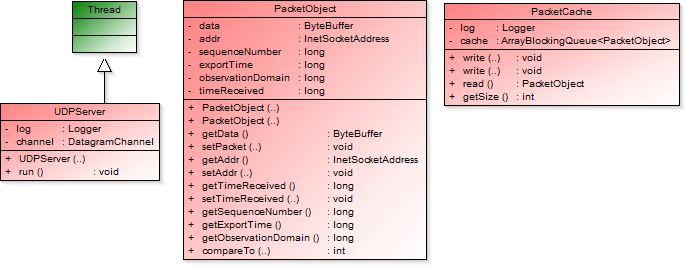
\includegraphics[width=1.0\textwidth]{collecting1_class}
\caption{Diagram tried prvej fázy zhromažďovacieho procesu}\label{o:collecting1_class}
\end{figure}

%%

Zjednodušený diagram tried druhej fázy sprostredkovateľského procesu je na Obr. \ref{o:collecting2_class}.

\begin{figure}[ht!]
\centering
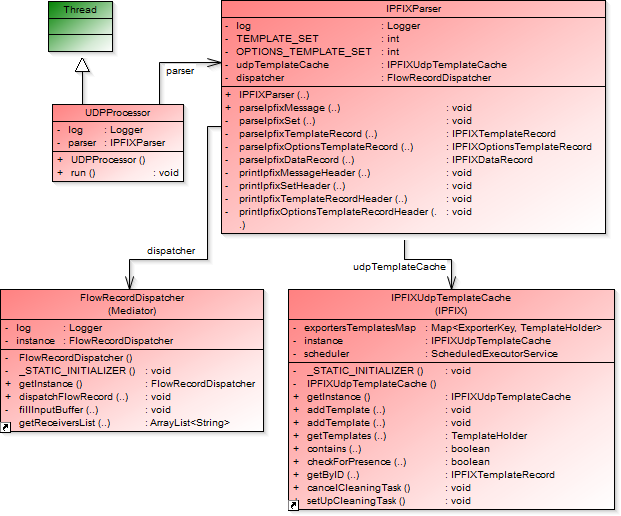
\includegraphics[width=1.0\textwidth]{collecting2_class}
\caption{Diagram tried druhej fázy zhromažďovacieho procesu}\label{o:collecting2_class}
\end{figure}

%%

Diagram tried rozhrania pre sprostredkovateľské procesy, vrátane triedy \verb|ExampleProcess| je znázornený
na obrázku \ref{o:intermediate_class}.

\begin{figure}[ht!]
\centering
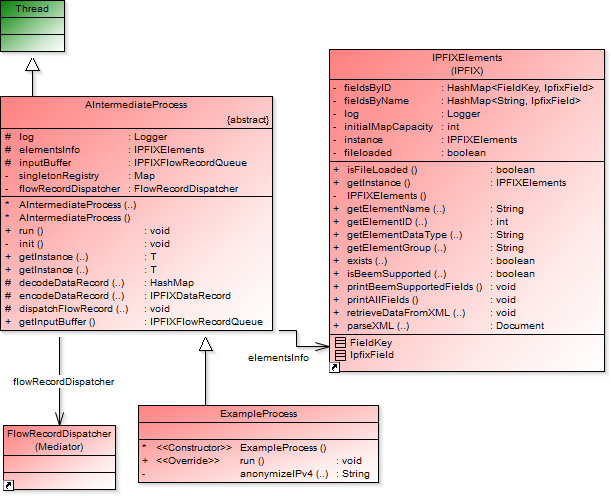
\includegraphics[width=1.0\textwidth]{intermediate_class}
\caption{Diagram tried rozhrania pre sprostredkovateľské procesy}\label{o:intermediate_class}
\end{figure}


%%

Diagram tried exportovacieho procesu.

\begin{figure}[ht!]
\centering
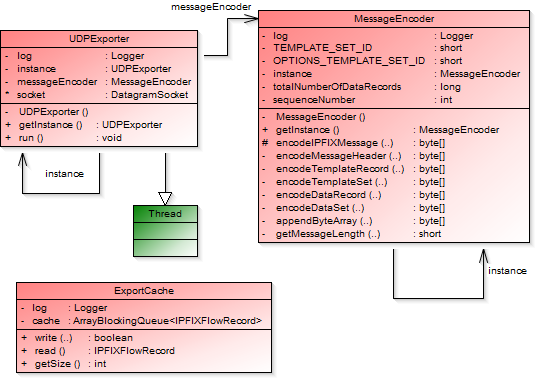
\includegraphics[width=1.0\textwidth]{exporting_class}
\caption{Diagram tried exportovacieho procesu}\label{o:exporting_class}
\end{figure}

%
% zivotopis autora
%\curriculumvitae\protect\label{page:posledna}
%Táto časť\/ je nepovinná. Autor tu môže uviesť\/ svoje biografické
%údaje, údaje o~záujmoch, účasti na~projektoch, účasti na~súťažiach,
%získané ocenenia, zahraničné pobyty na~praxi, domácu prax, publikácie
%a~pod.
%\kcurriculumvitae

\end{document}
%%